\documentclass[a4paper,fleqn,twoside]{book}
\usepackage{graphicx,amsmath,amsfonts,psfrag,fancyhdr,layout,appendix,xspace}
\usepackage[lofdepth,lotdepth]{subfig}
\usepackage[utf8]{inputenc}
\usepackage[spanish]{babel}
\usepackage{listings}
\usepackage{makeidx}
%\usepackage{ucs}
%\usepackage[utf8]{inputenc}
%\usepackage[T2A]{fontenc} %PROBANDO para RUSO
\usepackage[numbers]{natbib}
%\usepackage{hypernat} CAUSA PROBLEMAS AL COMPILAR - PROBLEMAS DE MUY DIFICIL LOCALIZACIÓN

%Para bibliogafía por capítulos con BibTeX
%\usepackage[sectionbib]{natbib}
%\usepackage{chapterbib}

%This change labels of subfig
%\renewcommand{\thesubfigure}{\alph{subfigure}\arabic{subfiggroup}}
\captionsetup[subfigure]{labelformat=simple,labelsep=colon, listofformat=subsimple}
%\captionsetup{lofdepth=2} This is in order to list the subfigures in the LOF
%\makeatletter
 %\renewcommand{\p@subfigure}{}
  %Esto lo agrego yo para tener subfiguras a1, b1, ... a2, b2, ... 
  %Se reinicia cada vez que una nueva figura es convocada (como es debido).
  %\newcounter{subfiggroup}[figure] 
%\makeatother


\usepackage{epsfig}
\usepackage{url}

%--------------------comandos para abreviar nombres---------------------

\newcommand{\s}{\textit{SQLite}\xspace}
\newcommand{\m}{\textit{MySQL}\xspace}
\newcommand{\p}{\textit{PostgreSQL}\xspace}
\newcommand{\cc}{\textit{crossdb}\xspace}
\newcommand{\jj}{\textit{JDBGM}\xspace}
\newcommand{\dd}{\textit{DBMS}\xspace}
\newcommand{\jd}{\textit{JDBC}\xspace}


\newcommand{\figpage}[1]{Figura~\ref*{#1} en la pagina~\pageref*{#1}}
\newcommand{\fullref}[1]{\ref{#1} de la página \pageref{#1}}

%--------------------Fin comandos para abreviar nombres---------------------

%Esto genera enlaces en el PDF
% \usepackage{html}
%Esto es para el conversor latex2html
\usepackage{color}
%\pagecolor{white}
\definecolor{lightgray}{rgb}{0.83,0.83,0.83}
\definecolor{darkgray1}{gray}{0.98}
\definecolor{darkgray}{gray}{0.40}
%Este mejora las prestaciones de "\verbatim"
%\usepackage{verbatim}
\usepackage{fancyvrb}
\fvset{gobble=2, frame=leftline, framesep=3mm, fontsize=\small, formatcom=\color{darkgray}}

\lstset{frame=shadowbox, rulesepcolor=\color{lightgray}, backgroundcolor=\color{darkgray1}, language=Java, numbers=left, numberstyle=\tiny, basicstyle=\footnotesize, xleftmargin= 
14pt}
%Definición de margenes
\usepackage[left=4.5cm,top=2.8cm,right=2cm,bottom=2.5cm]{geometry}
\sloppy
\pagestyle{empty}

% Code for creating empty pages
% No headers on empty pages before new chapter
\makeatletter
\def\cleardoublepage{\clearpage\if@twoside \ifodd\c@page\else
    \hbox{}
    \thispagestyle{plain}
    \newpage
    \if@twocolumn\hbox{}\newpage\fi\fi\fi}
\makeatother \clearpage{\pagestyle{plain}\cleardoublepage}

% Code for creating fully-empty pages
% Fully empty pages before command is called
\makeatletter
\def\clearfullypage{\clearpage\if@twoside \ifodd\c@page\else
    \hbox{}
    \thispagestyle{empty}
    \newpage
    \if@twocolumn\hbox{}\newpage\fi\fi\fi}
\makeatother \clearpage{\pagestyle{empty}\clearfullypage}

% Dutch style of paragraph formatting, i.e. no indents.
\setlength{\parskip}{1.3ex plus 0.2ex minus 0.2ex}
\setlength{\parindent}{0pt}

%\includeonly{edicion}
%\includeonly{jurado,apoyo,licencia,edicion,reconocimientos,tvs}

% Double space for REVISION
%\renewcommand{\baselinestretch}{2.0}

%Print subsubsection numbers and put them in TOC
\setcounter{secnumdepth}{3}
\setcounter{tocdepth}{3}

\makeindex

%Esto no dió resultado, se deseaba pasar 0.0 -> 0.0 y no -> 0,0
%Cambia el signo decimal a punto (en lugar del predeterminado: coma)
%\DeclareMathSymbol{.}{\mathpunct}{letters}{"3B}
%\DeclareMathSymbol{,}{\mathord}{letters}{"3B}
%\DeclareMathSymbol{\decimal}{\mathord}{letters}{"3A}

\usepackage[colorlinks=true, linkcolor= black ]{hyperref}

\begin{document}
%Cambiar Cuadros por Tablas y lista de... Debe ir después de \begin{document}
\renewcommand{\listtablename}{Índice de tablas} 
\renewcommand{\tablename}{Tabla} 


%%%%%%%%%%%%%
\frontmatter
%%%%%%%%%%%%%
%\ input{portada} %Se compila aparte y se junta con "gs".
%gs -dNOPAUSE -sDEVICE=pdfwrite -sOUTPUTFILE=tesiscompleta.pdf -dBATCH portada.pdf tesis.pdf
\pagestyle{empty}
%\ include{jurado}
\clearfullypage
\pagenumbering{roman}
%\ include{apoyo}
%\ input{licencia}
%\ include{edicion}
%\clearfullypage
%\ include{reconocimientos}
%\ include{russian}

% Define pagestyle
\pagestyle{fancy}
\fancyhf{}
\renewcommand{\chaptermark}[1]{\markboth{ \emph{#1}}{}}
\fancyhead[LO]{}
\fancyhead[LO]{}
\fancyfoot[LE,RO]{\thepage}

% Redefine plain page style
\fancypagestyle{plain}{
\fancyhf{}
\renewcommand{\headrulewidth}{0pt}
\fancyfoot[LE,RO]{\thepage}
}

% Dutch style of paragraph formatting, i.e. no indents.
\setlength{\parskip}{1.3ex plus 0.2ex minus 0.2ex}


% Remove parskip for toc
\setlength{\parskip}{0ex plus 0.5ex minus 0.2ex}

\tableofcontents
\listoffigures
\listoftables

%\cleardoublepage
%\ include{resumen} 
\cleardoublepage
%\ include{resumenen} 
% Adjustments headers
\fancyhead[RO]{\leftmark}

%%%%%%%%%%%%%
\mainmatter
%%%%%%%%%%%%%
\pagenumbering{arabic}
% Adjustments headers
\fancyhead[RO]{\leftmark}
\fancyhead[EL]{\emph{Capítulo \thechapter}}
%\setcounter{page}{3}

\chapter{Introducción}\label{capitulo:intro}
En cualquier sistema informático es común encontrarse con el uso de bases de datos relacionales para manejar, valga la redundancia, los datos que este debe procesar. Estos datos deben ser leídos, actualizados y registrado por el sistema en la base de datos, pero el sistema no es el que controla la base de datos si no que es el \textit{Sistema de Gestión de Base de Datos} o \textit{Motor de base de datos} o \textit{\dd}\footnote{Por sus siglas en ingles} el que controla la base de datos y cualquier acción que se quiera realizar sobre la base de datos se hace a través del motor mediante el lenguaje SQL, es decir el sistema informático debe comunicarse con el motor de base de datos.

En el mercado existen muchos \dd relacionales\footnote{Se usara \dd como sinónimo de \textit{RDBMS} a lo largo de todo el texto pero hay que tener en cuenta que \dd es un termino genérico que no se refiere solo a motores relacionales.} Microsoft SQL Server, MySQL y Oracle son solo algunos de ellos, esta amplia variedad crea algunos problema de compatibilidad puesto que cada uno de estos motores define un dialecto de SQL particular, muy a pesar de que SQL es un estándar de bastante antigüedad. El echo de por que se usan estos dialectos en vez del estándar corresponden a factores que no interesa discutir pero se puede nombrar como ejemplo la necesidad de mantener a los clientes atados a una plataforma en particular.

La comunicación con el motor se hace a través de un \textit{driver} que por lo general es provisto por el desarrollador del motor y es especifico para este dependiendo de la plataforma sobre la que se este trabajando. Entonces al desarrollar un sistema informático que utilice una base de datos,  se debe tener en cuenta que exista el \textit{driver} para el lenguaje de programación que se esta por utilizar y además que al desarrollar con un determinado motor el sistema queda atando en cierta medida al uso de este. Esta dependencia con el motor puede ser minimizada dependiendo de como se diseñe el sistema, en este sentido se debe pensar que el sistema debe concentrarse en los datos y no en como obtener los datos, por ejemplo se puede pensar el caso de un sistema de ventas, desarrollado bajo POO, en el que existe una clase \verb=Ventas= que se encarga de gestionar las ventas, las cuales es necesario que estén registradas en una base de datos, una primera solución sería que dicha clase se encargue de comunicarse con el motor y de grabar los datos, lo cual es posible pero se presentarían dos cuestiones: primero la clase perdería cohesión pues se estaría encargando de tareas extras y segundo la clase estaría interviniendo en el acceso al motor por lo que esta debería conocer mas cosas de la que debe, es decir habría un mayor acoplamiento entre las diferentes clases, estas cuestiones hacen a la dificultad de mantenimiento del software que es una clave importante para la subsistencia del mismo. Una segunda solución seria que otra clase se encargue de realizar la persistencia de los datos, de este modo \verb=Ventas= no tiene que conocer como es que se están persistiendo los datos solo necesita enviarle un mensaje a la otra clase y dejar que ella se encargue del trabajo. En el anterior ejemplo se estaría acentuando la dependencia con un motor en particular a la vez que se crear otros problemas, en cambio en la segunda solución se tiene una menor dependencia y se eliminan algunos problemas de diseño.

El presente trabajo pretende desarrollar en principio una capa de abstracción para manejar distintos motores de bases de datos desde el lenguaje Java ocultando los detalles correspondientes al acceso a cada motor en particular, inicialmente se dará soporte para 3 motores pero  la estructura de el componente permitirá agregar fácilmente soporte para mas motores. El nombre del proyecto es \textit{Java Data Base Generic Manager} o \jj que es como sera referido de aquí en mas.
%
%
\section{Objetivos generales}
El presente proyecto precisa que se realicen dos tareas básicas bien distintas, la primera es el estudio de los diferentes \dd para aprender como es que se manejan esos motores y poder conocer tanto las características en común como aquellas en las que difieran, la segunda tarea tiene que ver con estudiar el modo de diseñar el proyecto, es decir de que modo estará estructurado \jj para poder permitir una fácil ampliación y un fácil mantenimiento. Así se pueden enumerar los siguientes objetivos generales del proyecto:
\begin{enumerate}
\item Familiarizarse con la lectura de documentación de proyectos.
\item Investigar sobre el uso de patrones de diseño.
\item Investigar como se diseña una API\footnote{\textit{Application Programming Interface}}.
\end{enumerate}
%
\section{Tecnología utilizada}
El proyecto sera desarrollado sobre el lenguaje de programación Java y los motores de base de datos \m, \p y \s que son a los que inicialmente se les pretende dar soporte. Como herramientas para asistir el desarrollo se utilizara el entorno de desarrollo Eclipse que esta especializado en Java y que además agrega otras herramientas como por ejemplo la librería de pruebas unitarias JUnit. Por otro lado se usara el sistema de control de versiones Git que a pesar de que se puede integrar en Eclipse, se prefirió manejarlo de manera separada para poder aprender de manera mas profunda su uso. Para el desarrollo de este informe se uso Latex junto con el ``IDE'' Texmaker. Todo el proyecto se desarrollo sobre el sistema operativo Ubuntu principalmente por la familiaridad y facilidad de uso de las herramientas que se están utilizando sobre este tipo de sistemas, por ejemplo Git fue inicialmente creado para ser usado en entornos *nix\footnote{Aunque actualmente se lo puede usar en Windows/Linux/Mac}.
%
%\section{Contribución de este trabajo}
%
%
%
\section{Organización del trabajo}
%
El presente trabajo se organiza de la siguiente forma. El Capítulo 1 introduce a el objetivo de el trabajo y lo enmarca dentro de una tecnología determinada además de presentar los objetivos generales que se persiguen. El Capítulo 2 expone algunas de las herramientas existentes que resuelven desde distintos enfoques la problemática que ataca este trabajo, nombrando entre ellas ORM, generadores de código y otros. El Capítulo 3 introduce formalmente la problemática que se esta atacando e introduce el concepto de Patrones de Diseño para terminar introduciendo la solución que se propone. El Capítulo 4 es la especificación formal de la solución que se propone, para ello se divide el proyecto en dos módulos internos, un manejador de sentencias y un API para el acceso a motores de base de datos. El capitulo 5 documenta los aspectos importantes de el diseño sobre el que se construyo el proyecto, siguiendo para ello la división en dos módulos principales que se introdujo en el capitulo anterior. El Capítulo 6 documenta los pormenores, ajustes y correcciones que se tuvieron que hacer durante la implementación de el proyecto y finalmente se comenta el modo en que se realizaron las pruebas sobre el código escrito. Para terminar con los capítulos se escribió una breve reseña sobre los resultados que se obtuvieron de el proyecto y el trabajo a futuro que se espera realizar.

Como Apéndice de este informe se creo un manual de usuario que cubre los aspectos básicos de uso de la herramienta que se desarrollo y una descripción de una simple aplicación de ejemplo que muestra un uso practico de la herramienta.
\chapter{Antecedentes}

\chapter{JDBGM}
En este capitulo describiremos el proyecto propuesto por este trabajo, empezaremos por recordar la problemática expuesta en el capitulo \fullref{capitulo:intro} pero de una manera mas técnica, además enmarcaremos el proyecto en un escenario mas especifico definiendo un lenguaje sobre el cual se desarrollara y los \dd a los que se les dará soporte, para luego exponer la solución propuesta.

\section{El problema}
Como empezamos a describir en la introducción del capitulo \ref{capitulo:intro} la dificultad que encontramos al usar motores de bases de datos en el desarrollo de sistemas informáticos se traduce en problemas de mantenibilidad y portabilidad, veamos estos dos puntos por separado:
\begin{itemize}
\item Problemas en la portabilidad: Al utilizar un motor\footnote{Hablando de motores de bases de datos} en particular nos atamos en mayor o menor medida al uso de este según como hayamos diseñado el sistema, el mayor problema se traduce en las diferentes sintaxis para SQL que define cada \dd culpa de ello es muy probable que una sentencia valida para un motor no lo sea para otro, por lo tanto a la hora de querer migrar desde un motor a otro e inclusive a una versión mas nueva del mismo motor es necesario  ``actualizar'' las sentencias para que se apeguen a la sintaxis del motor al que se pretende migrar. Además como parte de su sintaxis particular cada \dd define sus propios tipos de datos lo que añade un poco mas de dificultad al proceso de cambio o migración desde un motor a otro.  
\item  Problemas en el mantenimiento: al utilizar bases de datos es importante como se diseña el acceso y manejo de los \dd, hay que tener en cuenta las siguientes cuestiones: quien se tiene que hacer cargo de la persistencia de los datos? El programa tiene que conocer los datos o mas bien como obtener los datos? Estas cuestiones no son nuevas y se solucionan en parte siguiendo patrones de diseño. Un ejemplo mas conciso de esto lo podemos ver cuando se esta diseñando un modulo de un sistema que precisa persistir ciertos datos en una BD, la pregunta que hay que hacerse es quien debería hacerse cargo de realizar esta persistencia? Si lo hace el modulo en si nos encontraríamos con accesos a la base de datos mezclados con la lógica de negocio del modulo además estos accesos implican que el modulo debe conocer como conectarse con la base de datos y de que modo se deben enviar y recibir los datos, con lo que nuestro modulo	perdería cohesión y ganaría complejidad derivando todo esto en una mayor dificultad en el mantenimiento.
\end{itemize}
Estos dos puntos están fuertemente relacionados pues la mantenibilidad del software esta muy ligada a la portabilidad y viceversa, esto por que la portabilidad hace a la mantenibilidad, pero cuando hablamos de que el software sea mantenible estamos hablando de muchos aspectos mas. Este trabajo esta centrado en el uso de la base de datos y como afecta esto a estos dos aspectos. Como ya se dijo es de buena practica el uso de patrones de diseño, así que en la sección siguiente veamos que es esto y como nos va a ayudar a encontrar una base para el proyecto. 
\section{Patrones de diseño}
Un patrón de diseño es una solución genérica y reusable  a un problema que ocurre de manera frecuente en un contexto dado. Un patrón de diseño no es un diseño terminado que pueda ser transformado directamente en código es mas bien una guía que indica como resolver un problema en determinados escenarios. Así los patrones de diseño son buenas costumbres que uno mismo debe implementar en la aplicación a desarrollar y en este mismo sentido son recomendaciones a tener en cuenta y no obligaciones\cite{Metsker:2002:DPJ}. Además es importante notar que el uso de patrones no garantiza éxito a la hora de diseñar. La descripción de un patrón indica cuando este puede ser aplicable, pero solo la experiencia nos hará comprender cuando el uso de un patrón de diseño en particular mejorara el diseño del software\cite{java:patrones}.


Entonces por que tener en cuenta a los patrones?
\begin{itemize}
\item Han sido provados. Los patrones reflejan la experiencia, conocimiento y perspectiva de desarrolladores quienes han aplicado satisfactoriamente estos patrones en su propio trabajo.

\item Son reusables. Los patrones proveen soluciones ya descubiertas que pueden ser aplicadas a diferentes problemas.

\item Son expresivos. Los patrones proveen un vocabulario común de soluciones que pueden expresar soluciones extensas de manera concisa.
%They are expressive. Patterns provide a common vocabulary of solutions that can express large solutions succinctly.
\end{itemize}
Existe mucha teoría sobre los patrones pero en este trabajo no nos interesa ahondar sobre ellos si no que interesaba introducir el concepto al lector para conocer un patrón que servirá de base para el desarrollo de \jj
\subsection{Data Acces Object}
Antes de describir este patrón tenemos que ubicarnos en un \textbf{contexto}, al acceso a los datos depende de la fuente de datos con la que se este trabajando. El acceso a almacenamiento persistente de datos, tal como una base de datos, varia fuertemente dependiendo del tipo de almacenamiento (BD relacionales, BD orientadas a objetos, archivos planos, etc) y de la implementación de un proveedor en particular.

El \textbf{problema} se da por que en cierto punto las aplicaciones necesitan persistir sus datos. Para muchas aplicaciones, la persistencia de los datos es implementada mediante diferentes mecanismos y hay marcadas diferencias en las API's usadas para acceder a estos diferentes mecanismos. Otras aplicaciones quizás necesite acceder a datos almacenados en diferentes sistemas muy distintos del cual se esta trabajando los cuales exigen utilizar sus APIs las cuales usualmente son propietarias. Esta disparidad entre las diferentes fuentes de datos produce desafíos en el diseño y además crea una potencial dependencia directa entre el código de la aplicación y el código de acceso a los datos. Dicha dependencia en el código de los componentes de la aplicación vuelve tediosa y dificultosa la migración desde un tipo de persistencia de datos a otra pues cuando cambia la fuente de datos el componente debe ser modificado para poder manejar la nueva fuente de datos.

La \textbf{solución} a este problema viene por usar un DAO (Data Acces Object) para abstraer y encapsular todos los accesos a la fuente de datos. DAO maneja la conexión con la fuente de datos para obtener y almacenar los datos.

EL DAO implementa los mecanismos de acceso necesarios para trabajar con la fuente de datos, esta fuente de datos puede ser un almacén de persistencia de cualquier tipo como por ejemplo un RDBMS, un servicio externo, un repositorio o incluso archivos xml. El componente del negocio (aquel que trabaja con la lógica del negocio) que se apoya en el DAO accede a la interfaz simplificada que este brinda para sus clientes. El DAO oculta completamente los detalles de la implementación de la fuente de datos a sus clientes y como la interfaz expuesta a los clientes del DAO no cambia cuando cambia la implementación de la fuente de datos este patrón permite que el DAO se adapte a diferentes esquemas de almacenamiento sin afectar sus clientes o componentes del negocio. Esencialmente el DAO actua como un adaptador entre el componente y la estructura de la fuente de datos.

% The DAO completely hides the data source implementation details from its clients. Because the interface exposed by the DAO to clients does not change when the underlying data source implementation changes, this pattern allows the DAO to adapt to different storage schemes without affecting its clients or business components. Essentially, the DAO acts as an adapter between the component and the data source.

La figura \ref{fig:dao-structure} muestra un diagrama de clases que muestras las relaciones en el patrón DAO.  

\begin{figure}
  \centering
    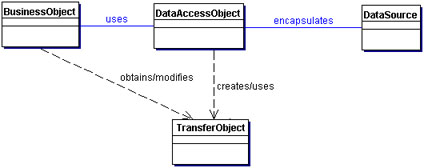
\includegraphics[width=0.6\textwidth]{figuras/dao-structure.jpg}
  \caption{Data Acces Object}
  \label{fig:dao-structure}
\end{figure}

Para finalizar nombremos las consecuencias de usar este patrón:
\begin{itemize}
\item Provee transparencia. El acceso a la fuente de datos es transparente pues los detalles de la implementación estan ocultos en el DAO. 


\item Facilita la migración.%Enables Easier Migration A layer of DAOs makes it easier for an application to migrate to a different database implementation. The business objects have no knowledge of the underlying data implementation. Thus, the migration involves changes only to the DAO layer. Further, if employing a factory strategy, it is possible to provide a concrete factory implementation for each underlying storage implementation. In this case, migrating to a different storage implementation means providing a new factory implementation to the application. 

\item Reduce la complejidad del código en los objetos que manejan la lógica del negocio. %Reduces Code Complexity in Business ObjectsBecause the DAOs manage all the data access complexities, it simplifies the code in the business objects and other data clients that use the DAOs. All implementation-related code (such as SQL statements) is contained in the DAO and not in the business object. This improves code readability and development productivity. 

\item Centraliza todo el acceso a los datos en una capa separada. %Centralizes All Data Access into a Separate Layer Because all data access operations are now delegated to the DAOs, the separate data access layer can be viewed as the layer that can isolate the rest of the application from the data access implementation. This centralization makes the application easier to maintain and manage. 

\item 
Not Useful for Container-Managed Persistence
% Because the EJB container manages entity beans with container-managed persistence (CMP), the container automatically services all persistent storage access. Applications using container-managed entity beans do not need a DAO layer, since the application server transparently provides this functionality. However, DAOs are still useful when a combination of CMP (for entity beans) and BMP (for session beans, servlets) is required. 


\item Agrega una capa extra, la cual debe ser diseñada e implementada para beneficiarse del uso de este patrón. %Adds Extra Layer The DAOs create an additional layer of objects between the data client and the data source that need to be designed and implemented to leverage the benefits of this pattern. But the benefit realized by choosing this approach pays off for the additional effort. 

\item Necesita diseño de jerarquía de clases, que implica otro esfuerzo extra. %Needs Class Hierarchy Design When using a factory strategy, the hierarchy of concrete factories and the hierarchy of concrete products produced by the factories need to be designed and implemented. This additional effort needs to be considered if there is sufficient justification warranting such flexibility. This increases the complexity of the design. However, you can choose to implement the factory strategy starting with the Factory Method pattern first, and then move towards the Abstract Factory if necessary.

\end{itemize}


\section{La solucion propuesta: \jj}
\chapter{Especificación}\label{capitulo:especificacion}
CAMBIAR INTRODUCCION!!!!!!!!!!!!!!11
En este capitulo describiremos detalladamente el proyecto y estableceremos los requisitos necesarios para cumplir con las necesidades que presentamos anteriormente, para ello se reseñara el modo en que Java accede a las bases de datos y explicare el modo en que se pretende ocultar este acceso dejando que \jj se encargue de los detalles de la conexión. Seguido a ello explicaremos como es que se pretende eliminar la dependencia del uso de los dialectos de SQL de cada motor.
%trabajando con mysql 5.1 reference manual\\

%trabajando con PostgreSQL 8.4 reference manual\\

%sqlite con el de la pagina la version 3\\

\section{Eliminando dialectos}
En el capitulo anterior se comento que parte del desafío de nuestro proyecto era lidiar con los diferentes  dialectos utilizados por cada motor por lo que a continuación analizaremos como es que JDBC trabaja con las sentencias SQL.

JDBC nos provee de la clase \verb=Statement=\footnote{Posteriormente explicare como es que se trabaja con JDBC por ahora interesa solo lo expuesto} la cual posee los metodos \verb=executeUpdate= y \verb=executeQuery= los cuales permiten enviar sentencias SQL al motor de base de datos.

Java ya nos provee JDBC para acceder a las bases de datos, pero al hacer uso de el es necesario especificar con que motor se esta trabajando, para ejemplificar ello veamos el típico código que debemos escribir para conectarnos a una base de datos.

\begin{lstlisting}[title=Porción de codigo java para la conexión a una base de datos]
class conectDB(){
...

Class.forName("com.mysql.jdbc.Driver");
	Connection conexion = DriverManager.getConnection(
		"jdbc:mysql://localhost/AsistenciaAlumnos", "tester",
		"tester");
	Statement st = (Statement) conexion.createStatement();

...
}
\end{lstlisting}

En esta porción de código lo que se hace inicialmente es instanciar el driver, es decir crear el objeto driver, luego el método estático \verb=getConnection= de 	\verb=DriverManager= nos devuelve un objeto que representa la conexión al motor con el que se esta trabajando. Este objeto del tipo \verb=Connection= nos provee métodos para generar objetos \verb=Statement= que nos permite hacer consultas a la base de datos mediante las funciones que dispone. Una descripción mucho mas extensa de JDBC puede ser encontrada en la documentación disponible en la web de Oracle\citep{java:jdbc}.
Para nuestro proyecto necesitamos ocultar y simplificar el API de JDBC





\section{JDBC y su envoltorio}
y otro






\section{Abstracción de SQL}
Uno de los problemas al intentar portar código SQL entre diferentes motores de bases de datos reside en que cada motor usa su propio dialecto de SQL. Las diferencias entre estos dialectos puede ser mínima pero aun así esto provoca que a una aplicación a la que se le quiera cambiar el motor de base de datos que usa actualmente se le deban revisar todas las sentencias SQL usadas.\\
Así que para brindar una abstracción sobre la base de datos es necesario que las consultas SQL (sin hacer diferencias sobre DDL \footnote{Data Definition Lenguaje} y DML \footnote{Data Manipulation Lenguaje}) no sean manejadas de forma explicita es decir que no seria conveniente, por ejemplo, manejar las consultas como cadenas de caracteres ya que esta es una estructura estática dependiente del DBMS que se este usando. Por lo que para poder manejar adecuadamente las consultas se considero usar una estructura de datos un poco mas compleja que contenga la consulta de manera desglosada. Es decir que en ves de tener una sentencia como la siguiente:
\begin{Verbatim}
  nombre_comando [opcion1 parametro1] [opcion2 parametro2] parametro; 
\end{Verbatim}

Se tendría una estructura de datos como la siguiente:

%\lstset{frame=single, rulesepcolor=\color{black}, backgroundcolor=\color{lightgray}, language=java, numbers=left, numberstyle=\tiny, basicstyle=\footnotesize}
\begin{lstlisting}[title=Pseudocódigo de la estructura de dato que contiene la sentencia]
class Sentencia{
	nombre_comando;
	parametro;
	opcion1(parametro1);
	opcion2(parametro2);
	devolver_sentencia();
}
\end{lstlisting}

Hay que tener en cuenta que el tipo de datos que se quiere manejar aparte de contener los parámetros de la sentencia debe brindar métodos para armar la sentencia, asignarles valores a los atributos y ser capaz de definir el comportamiento especifico que pueda tener la sentencia. Cuando se dice que el tipo de dato, mas en concreto la clase, que represente la sentencia sea capaz de armar la sentencia se refiere a que sea capaz de devolver la cadena de caracteres que represente una sentencia SQL valida para algún DBMS.\\
Así podemos hacer un resumen de las características que se desea cumplan estas estructuras:
\begin{enumerate}
	\item La estructura debe devolver una cadena de caracteres (un \textit{String}) que represente una sentencia SQL valida para el \dd deseado.
	\item Cada sentencia  SQL debe estar representada por una estructura diferente pero similar a las demás para que el armado de las sentencias mediante estas estructuras sea consistente, de modo que la sintaxis usada sea sencilla de aprender. 
	\item La estructura debe contemplar que no se realicen acciones no permitidas con las sentencias, ya que si bien las acciones disponibles estarán limitadas por la estructura en si hay algunas otras opciones que pueden ser excluyentes con otras, esto se debe controlar.
	\item La estructura debe contemplar todas las opciones disponibles para las sentencias que se están por incluir.
\end{enumerate}
Sobre este ultimo punto hay que aclarar que solo se cubrirá un subconjunto de todas las sentencias posibles que define SQL. Este conjunto estará formado por:
\begin{enumerate}
\item CREATE TABLE - Permite crear tablas 
\item ALTER TABLE - Modifica la estructura de una tablas \footnote{Solo se da un soporte básico para esta sentencia}
\item UPDATE - Modifica las filas de una tabla 
\item INSERT - Inserta nuevas filas a una tabla
\item DELETE - Elimina columnas de una tabla
\item SELECT - Realiza consulta sobre las tablas
\end{enumerate}

%Se agruparon las sentencias de acuerdo a el resultado que producen, por un lado tenemos a las sentencias que devuelven datos mas allá de una información que indique el éxito o fracaso de la interpretación de la sentencia en el DBMS o sea sentencias como SELECT, por otro lado tenemos aquellas que solo devuelven información del exito o fracaso de la interpretación de la sentencia.
Una vez definido el subconjunto de sentencias con las que se trabajaran es necesario que para cada una de ellas se defina un comportamiento común, es decir que estaremos definiendo un nuevo dialecto de SQL el cual sera soportado por todos los \dd, pero para que esto sea posible deberemos restringir las dialectos soportados al que menos posibilidades presente o viéndolo de otro modo es necesario extraer un dialecto común a todos ellos. Además de las sentencias es necesario tener en cuenta los tipos de datos que se usan en cada \dd también para ellos debemos encontrar un factor común, por lo que a continuación analizamos los tipos de datos usados por cada motor, luego se hará un análisis por separado para cada una de las sentencias elegidas.



\subsection{Tipos de datos y sus diferencias}
Las primeras diferencias las encontramos en las definiciones de tipos de datos que usan los \dd, de estas la mas notoria es el modo en que \s maneja los tipos de datos. La mayoría de los motores de datos manejan un tipo de datos estático, en el que el contenedor del dato (la columna) define el tipo de dato que podrá almacenar, o sea el tipo declarado de dato en la definición de la columna. En cambio en \s no existen los tipos de datos como tal, si no que definieron las clases de almacenamiento\cite{sqlite:datatypes} (\textit{storage clases}) que son mas genéricas que los tipos de datos definidos usualmente, por ejemplo la clase de almacenamiento \verb=INTEGER= puede almacenar 6 diferentes tipos de datos enteros con diferentes longitudes, que es en definitiva en lo que difieren por ejemplo los tipos de datos \verb=SMALLINT= e \verb=INTEGER=, que maneja \m.\\

 En \s el tipo de dato de un valor esta asociado a el dato en si y no a su contenedor, pero aun así existe compatibilidad con los otros motores en el sentido de que \s puede interpretar adecuadamente sentencias SQL validas que usen los clásicos tipos de datos estáticos. Para brindar esta compatibilidad se define el concepto de afinidad de tipo para las columnas que viene a ser el tipo de dato recomendado para los datos almacenados en esa columna, así existe una serie de reglas para definir la afinidad de la columna en base a el nombre del tipo de dato declarado para esa columna, pudiendo ser este nombre cualquiera. Aun así la afinidad de la columna \textbf{recomienda} un tipo de dato no lo exige para esa columna, por lo que en \s una columna puede almacenar cualquiera de los tipos de datos definidos (storage class para \s).\\
 
\cc debe proveer una interfaz única en la que se establezcan los tipos de datos disponibles para usar, estos tipos de datos deben ser elegidos en base a las compatibilidades entre los diferentes motores que soporta para lograr un uso genérico sobre cualquiera de los motores, en principio se podrían elegir todos los tipos de datos definidos en los motores, uniendo a aquellos que sean equivalentes en un solo tipo y dejando que después \cc se encargue de mapear los datos a los soportados por un motor en concreto, recordando que algunos de los datos declarados no son directamente soportados por todos los \dd. Pero esto podría acarrear confusiones pues veamos, el tipo de dato entero mas chico (el que ocupa menos espacio en disco para representarse) en \m\cite{mysql:datatypes} es \verb=TINYINT= que ocupa solo 1 byte, en cambio en \p\cite{postgre:datatypes} el mas chico es \verb=SMALLINT= que ocupa 2 bytes entonces en el caso de que en los tipos de datos especificados para \cc se encuentren estos dos no habría problemas al usarlos pues si se llegara a especificar una columna con tipo de dato \verb=TINYINT= mientras se trabaja sobre una base de datos con \p no habría mas que mapear internamente el tipo de dato a \verb=SMALLINT=, pero en esta situación el programador podría no enterarse de que en realidad la columna que el esta usando ocupa 2 bytes por dato lo que en casos en que el espacio en disco duro sea un tema sensible podría llevar a serias confusiones, entonces lo mejor es que en la especificación de \cc solo se incluyan los tipos que no lleven a este tipo de confusiones. A continuación se analizan los tipos de datos y sus congruencias, empezando por los datos numéricos del tipo entero mediante un cuadro comparativo:
        
\begin{table}[h]
\begin{center}
\begin{tabular}{|c|c|c|}
\hline \s      & \m        & \p \\ 
\hline         & TINYINT   &  \\ 
               & SMALLINT  & SMALLINT \\ 
       INTEGER & MEDIUMINT &  \\
               & INT       & INTEGER \\
               & BIGINT    & BIGINT \\  
\hline 
\end{tabular} 
\end{center}
\caption{Comparación de los tipos de datos enteros}
\end{table}

Como podemos ver la clase de almacenamiento \verb=INTEGER= de \s es capaz de contener todos los tipos de datos declarados en los otros dos motores, en \m se definen mas tipos de datos enteros que  difieren únicamente en el espacio que utiliza para almacenarse en disco, el mas chico usa  solo 1 Byte para almacenarse, mientras que el mas grande usa 8 Bytes. En \s el dato es almacenado en disco con la menor cantidad posible de Bytes pero tan pronto como es cargado en memoria es convertido a un entero de 8 bytes con signo\footnote{Cuando al representarse un numero se usa el signo ($\pm$) se achica el rango de numero que se puede representar}. Lo que nos  interesa a nosotros es elegir un subconjunto de estos tipos que sean aplicables a los tres motores, en este caso es \p el que define menos tipos de datos, teniendo en cuenta que \s presenta un tipo de dato que envuelve a todos los demás, por lo que tomaremos esos tipos como los elegidos para \jj

\begin{table}[h]
\begin{center}
\begin{tabular}{|c|c|c|}
\hline \s   & \m               & \p \\  
\hline      & FLOAT            &  \\ 
       REAL & REAL             & REAL \\
            & DOUBLE PRECISION & DOUBLE PRECISION \\
\hline 
\end{tabular} 
\end{center}
\caption{Comparación de los tipos de datos reales aproximados}
\end{table}

En el caso de los tipos de números reales tenemos básicamente dos clases de tipos, los que guardan los datos de forma exacta y otros no exactos que se guardan en el formato punto flotante. Para el caso de los tipos de datos con punto flotante tomare los datos definidos para \p como los elegidos para \cc, el tipo \verb=FLOAT= definido en \m es similar a \verb=REAL=, y nuevamente el tipo \verb=REAL= de \s es capaz de contener los otros tipos. 

\begin{table}[h]
\begin{center}
\begin{tabular}{|c|c|c|}
\hline \s & \m & \p \\  
\hline  & NUMERIC & NUMERIC \\
  & DECIMAL & DECIMAL \\
NUMERIC  & DATETIME &  \\
  & TIMESTAMP & TIMESTAMP \\
  & DATE & DATE \\
  & TIME & TIME \\  
\hline 
\end{tabular} 
\end{center}
\caption{Comparación de los tipos de datos reales exactos y fechas}
\end{table}

Para analizar el caso de los tipos de datos reales con almacenamiento exacto, deberemos analizar los tipos de datos de fecha y hora, pues aunque parezca un poco confuso \s no tiene un tipo de dato especifico para estos tipos, pero si posee una afinidad de columnas para ellos que se denomina, \verb=NUMERC=, este afinidad lo que hace es decidir cual es el mejor modo de almacenar el dato, pudiendo ser cualquier de las clases \verb=NULL, INTEGER, REAL, TEXT= y \verb=BLOB=. Para los tipos \verb=NUMERIC= Y \verb=DECIMAL= que son para almacenamiento exacto de números reales no tenemos una clase especifica, pero lo que si podemos hacer es asignarle el tipo (afinidad de columna) \verb=NUMERIC= que se encargara de que el motor guarde el dato en el formato que le parezca mas adecuado. Para los datos del tipo fecha y hora tenemos bastante similitud  en \m y \p salvo que en \m esta \verb=DATETIME= que en lo unico que difiere de \verb=TIMESTAMP= es en el rango de fechas que soporta. En \s no tenemos tipos de datos para fecha y hora, pero se pueden guardar las fechas como cadenas de texto o numero, por lo que si se le da la afinidad de columna \verb=NUMERIC= el motor resolver cual es el mejor tipo de datos para almacenar la facha u hora según el formato que estemos utilizando.   

\begin{table}[h]
\begin{center}
\begin{tabular}{|c|c|c|}
\hline \s & \m & \p \\ 
\hline  & CHAR(n) & CHAR(n) \\  
    & VARCHAR(n) & VARCHAR(n) \\ 
  TEXT   & TINYTEXT &  \\  
    & TEXT & TEXT \\  e{wiki:xxx}
    & MEDIUMTEXT &  \\  
    & LONGTEXT &  \\  
\hline 
\end{tabular} 
\end{center}
\caption{Comparación de los tipos de datos cadenas de texto}
\end{table}

Para el caso de los tipos de datos tenemos como siempre \s con una clase de almacenamiento bastante genérica que cubre todos los tipos de datos definidos en los demás motores. La diferencia que encontramos con los otros dos motores es que el tipo \verb=TEXT= que en \m tiene 4 variantes que varían en el limite de almacenamiento, siendo el ultimo sin limite (\verb=LONGTEXT=) en cambio en \p existe solo \verb=TEXT= y que es para almacenamiento de texto sin limite, así que como antes tomaremos los tipos de datos que define \p como los elegidos para \cc. 

\begin{table}[h]
\begin{center}
\begin{tabular}{|c|c|c|}
\hline \s & \m & \p \\ 
\hline  & BINARY &  \\  
 & VARBINARY &  \\ 
 BLOB & TINYBLOB & bytea \\ 
 & BLOB &  \\ 
 & MEDIUMBLOB &  \\
& LONGBLOB &  \\ 
\hline 
\end{tabular} 
\end{center}
\caption{Comparación de los tipos de datos binarios}
\end{table}

En el caso de los tipos de datos binarios tenemos.
Faltan los tipos monetarios, booleanos

\begin{table}[h]
\begin{center}
\begin{tabular}{|c|c|c|}
\hline \s & \m & \p \\ 
\hline 1 o 0 & 1 o 0 & BOOLEAN \\  
\hline NUMERIC & NUMERIC & MONETARY \\  
&  &  \\  
\hline 
\end{tabular} 
\end{center}
\caption{Comparación de tipos de datos varios}
\end{table}

\subsection{Funciones}





\subsection{Diseño de CREATE TABLE}
Esta sentencia es usada para crear tablas en una base de datos relacional, un resumen de su sintaxis como se la define en el estándar SQL es la siguiente:
\begin{Verbatim}
  CREATE TABLE <table name> (
  { <column name> [ <column type> ][ PRYMARY KEY ][ REFERENCES <foreign table> ] }...
  )
  [ PRIMARY KEY <indexed columns> ]
  [ FOREIGN KEY <columns and referenced table> ]
\end{Verbatim}
Se obviaron las definiciones de algunas de las opciones de\verb= CREATE TABLE= puesto que escapan al alcance del proyecto el cual esta limitado por los DBMS a los que tiene que soportar además hay que tener en cuenta algunas salvedades, como que si se especifica una columna como\verb= PRIMARY KEY= dentro de la definicion de la columna no se puede especificar la clausula\verb= PRIMARY KEY= fuera de los paréntesis que encierran a las definiciones de las columnas. Mas específicamente podemos empezar con \s el cual, sin restarle importancia, es el que menos características implementa debido a su "pequeñez" por lo cual pasamos a estudiar\verb= CREATE TABLE= tal como la entiende \s\footnote{para ver la sintaxis usada ir a QQQQQQQQ} y comparando las diferencias con \m y \p:

\begin{Verbatim}[frame=leftline, framesep=3mm]
  CREATE [ TEMP | TEMPORARY ] TABLE <database name> <dot> <table name> 
  [ IF NOT EXISTS ] <table contents source>

  <table contents source> ::=
    <left paren> <table element> [ { <comma> <table element> }... ] <right paren>
  | AS <select stmt>
\end{Verbatim}

Los parámetros\verb= TEMPORARY= y\verb= TEMP= se usan indistintamente para crear una tabla temporaria en \s, lo cual es soportados por los 3 DBMS con la salvedad que en \m solo se acepta la palabra reservada\verb= TEMPORARY=. El parámetro\verb= IF NOT EXISTS= indica que de existir una tabla del mismo nombre la sentencia \verb= CREATE TABLE= no tiene efecto sobre la base de datos, este parámetro no es soportado por \p por lo que sera omitido. Por ultimo hay que tener en cuenta que al ser \s un motor "serverless" siempre se esta trabajando o sobre la base de dato principal o sobre una temporaria por lo que este para el parámetro\verb= <database name>= solo acepta\verb= "main"= ó\verb= "temp"= de modo que en un principio el nombre de la base de dato no se tomara en cuenta y cualquier tabla que se cree sera en la base de dato actual.

\begin{Verbatim}
  <table element> ::=
    <column definition>
  | <table constraint definition>

  <column definition> ::=
  <column name> [ <data type> | <domain name> ]
  [ DEFAULT <default option> ]
  [ <column constraint definition>... ]
  [ COLLATE <colation name> ]

  <default option>::=
    <signed number>
  | <literal value>
  | <left paren> <expr> <left paren>
  
  <column constraint definition> ::=
  [ CONSTRAINT <name> ] <column constraint>

  <column constraint> ::=
    NOT NULL <conflict cause>
  | UNIQUE <conflict cause>
  | PRIMARY KEY [ ASC | DESC ] <conflict cause> [ AUTOINCREMENT ]
  | <references specification>
  | CHECK <left paren> <expr> <right paren>
\end{Verbatim}

La siguiente sección a estudiar es la definición de columnas y restricciones de columna que se diferencian de las restricciones de tabla en que las primeras se definen junta a la definición de columna y solo se pueden hacer sobre una única columna, en cambio las restricciones de tabla se hacen después de las definiciones de columnas y estas pueden referirse a un grupo de columnas.\\

Como primer diferencia veremos las tipos de datos tienen diferentes nombres y significados, pero esto sera tratado mas adelante\footnote{referenciar a alguna parte de la tesis}. La clausula\verb= DEFAULT= en este caso esta limitada por \m que solo acepta valores constantes, es decir no se podria usar funciones como \verb= NOW()= con la excepción de que se puede poner\verb= CURRENT_TIMESTAMP= como\verb= DEFAULT= para una columna del tipo\verb= TIMESTAMP=.\\

El parámetro\verb= COLLATE= también presenta diferencias, pero es en este caso es \p el que limita ya que no acepta\verb= COLLATE= en la definición de columna por lo que no sera adoptada en la especificación de \cc. En \p se puede especificar el ``collate'' a usar sobre todas las tablas en la creación de la base de datos. \verb= UNIQUE= y \verb= PRIMARY KEY= como restricción de columna no acepta ningún modificador en \m, por lo tanto se obviara el modificador\verb= <conflict cause>= de\s y otros que acepta \p. El parametro \verb= NOT NULL= tampoco acepta ningún modificador en \m, su contra parte el parámetro\verb= NULL= puede ser omitido ya que de no agregarse se toma por defecto que la columna puede aceptar valores nulos. Por ultimo hay que señalar que \m si bien implementa\verb= CHEK <expre>= este no es reconocido en la definición de columna.\\

En \s y \p a las restricciones de columna se les puede especificar un nombre con \verb=CONSTRAINT <name>= pero esto no es soportado en \m una ultima diferencia la podemos ver en el parámetro\verb= AUTOINCREMENT= (\verb=AUTO_INCREMENT= en \m) que solo se puede especificar cuando una columna es\verb= PK= y del tipo \verb= INTEGER=, en \m se puede hacer incluso sobre columnas que no sean \verb=PK=, en \p este parámetro no existe, al menos no en la version  sobre la que se esta trabajando.  

\begin{Verbatim}
  <table constraint definition> ::=
  [ CONSTRAINT <name> ] <table constraint>

  <table constraint> ::=
    [ UNIQUE | PRIMARY KEY ] <left paren> <unique column list> <right paren> <conflict cause>
  | <referential constraint definition>
  | CHECK <left paren> <expr> <right paren>

  <unique column list> ::= <column name list>

  <referential constraint definition> ::=
  FOREIGN KEY <left paren> <referencing columns> <right paren>
  <references specification>
\end{Verbatim}

De las restricciones de tabla la única a la que no se le podrá especificar un nombre de restricción con \verb=CONSTRAINT <name>= es la restricción \verb=CHECK (expr)=. Los parámetros \verb=UNIQUE= y \verb=PRIMARY KEY= que se especifican como restricción de tabla solo comparten en común entre la especificación de los 3 DBMS que encierran entre paréntesis a las columnas que se indican con dicha restricción. Resta por analizar la especificación de clave foránea (\verb=FK=):    

\begin{Verbatim}
  <references specification> ::=
  REFERENCES <referenced table and columns>
  [ MATCH { FULL | PARTIAL | SIMPLE } ] [ <referential triggered action> ]
  [ <constraint characteristics> ]

  <referenced table and columns> ::=
  <table name> [ <left paren> <reference column list> <right paren> ]

  <reference column list> ::= <column name list>

  <referential triggered action> ::=
    <update rule> [ <delete rule> ]
  | <delete rule> [ <update rule> ]

  <update rule> ::= ON UPDATE <referential action>

  <delete rule> ::= ON DELETE <referential action>

  <referential action> ::=
    CASCADE
  | SET NULL
  | SET DEFAULT
  | RESTRICT
  | NO ACTION

   <constraint characteristics> ::=
  [ NOT ] DEFERRABLE [ INITIALLY DEFERRED | INITIALLY IMMEDIATE ]
\end{Verbatim}
Los parámetros \verb=MATCH { FULL | PARTIAL | SIMPLE }= son reconocidos en los 3 DBMS, pero en \s no tienen ningún efecto, es decir que estos se pueden especificar pero siempre se tendra que la \verb=FK= se procesara con \verb=MATCH SIMPLE=, con lo que de momento sera parte de la especificación pero hay que tener siempre en cuenta que \s lo procesara de manera diferente. Por ultimo quedan dos diferencias, la primera es que la opción \verb=SET DEFAULT= de \verb=<referential action>= no es soportada por \m; segundo que \verb=<constraint characteristics>= no es soportada por \m.\\

%------------------------TODO-----------------------------------
%revisar lo de SET DEFAULT!!!!!!!!!!!!!!!!!!!!!!!!!!!!!!!!!!!!!!!!!!!!!!!!!!!!


%----------------------------Especificación de CREATE TABLE------------

Así que finalmente tenemos las siguiente sintaxis de \verb=CREATE TABLE= para el proyecto\\

\begin{Verbatim}[frame=single, label=sintaxis para CREATE TABLE]
  CREATE [ TEMPORARY ] TABLE <database name> <dot> <table name> 
  <table contents source>

  <table contents source> ::=
    <left paren> <table element> [ { <comma> <table element> }... ] <right paren>
  | AS <select stmt>
  
  <table element> ::=
    <column definition>
  | <table constraint definition>

  <column definition> ::=
  <column name> [ <data type> | <domain name> ]
  [ DEFAULT <constant> ]
  [ <column constraint>... ]
  
  <column constraint> ::=
    NOT NULL
  | UNIQUE
  | PRIMARY KEY
  | <references specification>

  <table constraint definition> ::=
  [ CONSTRAINT <name> ] <table constraint>

  <table constraint> ::=
    [ UNIQUE | PRIMARY KEY ] <left paren> <unique column list> <right paren>
  | <referential constraint definition>
  | CHECK <left paren> <expr> <right paren>

  <unique column list> ::= <column name list>

  <referential constraint definition> ::=
  FOREIGN KEY <left paren> <referencing columns> <right paren>
  <references specification>
  
  <references specification> ::=
  REFERENCES <referenced table and columns>
  [ MATCH { FULL | PARTIAL | SIMPLE } ] [ <referential triggered action> ]

  <referenced table and columns> ::=
  <table name> [ <left paren> <reference column list> <right paren> ]

  <reference column list> ::= <column name list>

  <referential triggered action> ::=
    <update rule> [ <delete rule> ]
  | <delete rule> [ <update rule> ]

  <update rule> ::= ON UPDATE <referential action>

  <delete rule> ::= ON DELETE <referential action>

  <referential action> ::=
    CASCADE
  | SET NULL
  | RESTRICT
  | NO ACTION


\end{Verbatim}




\subsection{Diseño de UPDATE}
DMS\\

Esta sentencia es usada para actualizar los datos de una tabla, es decir para modificar valores existentes de filas. El análisis de la siguiente sintaxis corresponde a como es entendida la sentencia \verb=UPDATE= por \s: 

\begin{Verbatim}
  <update statement> ::=
  UPDATE [ OR <or option> ] <target table> 
  SET <set clause list>
  [ WHERE <search condition> ]
  
  <or option> ::=
    ROLLBACK
  | ABORT
  | REPLACE
  | FAIL
  | IGNORE
\end{Verbatim}

En este punto encontramos la primer diferencia con los demas DBMS, el elemento \verb=<or option>= que nos permite especificar que acción tomar si no es posible realizar la acción de \verb=UPDATE= sobre la tabla, es un añadido de \s que no esta presente en las especificaciones de los otros dos DBMS y tampoco aparece en la especificación de SQL.

\begin{Verbatim}
  <target table> ::=
  [ <database name> <dot> ] <table name>
  [ INDEXED BY <index name> ]
  [ NOT INDEXED ]
  
  <set clause list> ::= <set clause> [ { <comma> <set clause> }... ]

  <set clause> ::=
  <column name> <equals operator> <expr>
  
  -----ONLY AVALAYBLE IF ACTIVATED DURING COMPILATION---------
  
  ORDER BY ... completar

\end{Verbatim}
Las elementos \verb=[ INDEXED BY <index name> ]= y \verb=[ NOT INDEXED ]= no son reconocidos por \m y \p por lo que serán ignorados en la especificación de el proyecto. Lo demás es de idéntica sintaxis. La especificación final de \jj.

\begin{Verbatim}[frame=single, label=sintaxis para UPDATE]
  <update statement> ::=
  UPDATE <target table> 
  SET <set clause list>
  [ WHERE <search condition> ]
  
  <target table> ::=
  [ <database name> <dot> ] <table name>
  
  <set clause list> ::= <set clause> [ { <comma> <set clause> }... ]

  <set clause> ::=
  <column name> <equals operator> <expr>    
\end{Verbatim}




\subsection{Diseño de INSERT}
La sintaxis que analizo a continuación corresponde a la sentencia \verb=INSERT= que sirve para insertar filas nuevas en una tabla dada, felizmente la sentencia de \verb=INSERT= entendida por \s solo difiere en dos aspecto de las otras, primero es que esta presenta el elemento \verb=<or option>= que no es soportado por los otros DBMS, segundo el elemento \verb=REPLACE= que tampoco es reconocido por los demas motores. Además es bueno aclarar que \s esta restringiendo las capacidades de los otros motores, como por ejemplo en \m existe el elemento \verb=ON DUPLICATE KEY UPDATE= el cual sirve para resolver conflictos cuando una insercción en una tabla provoca que alguna columna que deba ser única (\verb=PK= ó \verb=UNIQUE=) presente un valor duplicado. Así que sin mas la siguiente es la sintaxis elegida y compatible con los tres motores:

\begin{Verbatim}[frame=single, label=sintaxis para INSERT]
  <insert statement> ::=
  INSERT INTO <insertion target> <insert columns and source>

  <insertion target> ::= [ <database name> <dot> ] <table name>

  <insert columns and source> ::=
    <from subquery>
  | <from constructor>
  | DEFAULT VALUES

  <from subquery> ::=
  [ <left paren> <insert column list> <right paren> ]
  <query expression>
  
  <from constructor> ::=
  [ <left paren> <insert column list> <right paren> ]
  VALUES <left paren> <exp> [ { <comma> <exp> }... ] <right paren>

  <insert column list> ::= <column name list>
\end{Verbatim}




\subsection{Diseño de ALTER TABLE} \label{sec:altertable}
\verb=ALTER TABLE= sirve en SQL para alterar la estructura de las tablas, en este caso nos encontramos con que \s esta limitando a los demás motores pues la sintaxis que soporta esta muy limitada, las únicas acciones que soportan son renombrar las tablas y agregar nuevas columnas a una tabla. Por lo que la sintaxis final elegida es la misma que soporta \s:\\

%\begin{Verbatim}
%  <alter table statement> ::= 
%  ALTER TABLE [ <database name><dot> ] <table name> <alter table action>
%  
%  <alter table action> ::=
%    RENAME TO <new table name>
%  | ADD [ COLUMN ] <column def>
%\end{Verbatim}
\begin{Verbatim}[frame=single, label=sintaxis para ALTER TABLE]
<alter table statement> ::= 
  ALTER TABLE [ <database name><dot> ] <table name> <alter table action>
  
  <alter table action> ::=
    RENAME TO <new table name>
  | ADD [ COLUMN ] <column def>
\end{Verbatim}

Además de estas limitaciones hay algunas mas, al agregar nuevas columnas la definición de estas puede tomar cualquiera de las opciones disponibles en la definición de \verb=CREATE TABLE= excepto por las siguientes:

\begin{enumerate}

\item La columna no puede ser clave primaria o \verb=UNIQUE=.

\item La columna no puede tener como valor por defecto \verb=CURRENT_TIME=, \verb=CURRENT_DATE=, \verb=CURRENT_TIMESTAMP=, o una expresión entre paréntesis.

\item Si la columna no puede tener valor nulo se ha de especificar un valor por defecto diferente de \verb=NULL=

\item If foreign key constraints are enabled and a column with a REFERENCES clause is added, the column must have a default value of NULL.

\end{enumerate}



\subsection{Diseño de DELETE}
La sintaxis de \verb=DELETE= entendida por \s es la siguiente
\begin{Verbatim}
  <delete statement> ::=
  DELETE FROM <target table> [ WHERE <search condition> ]

  <target table> ::=
  [ <data base name><dot> ] <table name>
  [ INDEXED BY <index name> ]
  [ NOT INDEXED ]
\end{Verbatim}
En ella podemos encontrar una diferencia con las demás motores de bases de datos, elementos que serán omitidos. Esta diferencia es que no es posible usar los elementos \verb=INDEXED BY <index name>= y \verb=NOT INDEXED= en \p y \m, además cabe aclarar que no se están agregando elementos que si son soportados por los otros motores. Así que finalmente nos queda la siguiente sintaxis:


\begin{Verbatim}[frame=single, label=sintaxis para DELETE]
  <delete statement> ::=
  DELETE FROM <target table> [ WHERE <search condition> ]
  
  <target table> ::=
  [ <data base name><dot> ] <table name>
  
\end{Verbatim}




\subsection{Diseño de SELECT}
Esta sentencia es quizá la mas compleja a analizar debido a la cantidad de posibilidades que presenta así sin mas analizamos a continuación \verb=SELECT= tal como es conocido por \s:

\begin{Verbatim}
  <query specification> ::=
  <select core> [ { <compound operator> <select core> }... ]
  [ ORDER BY <ordering term> [ { <comma> <ordering term> }... ]
  [ LIMIT <expr> [ { OFFSET | <comma> } <expr> ] ]  
\end{Verbatim}

Hasta este punto la sintaxis usada es compatible con los otros dos motores, por lo que sera aceptada tal cual, así que se siguen buscando diferencias:

\begin{Verbatim}
  <select core> ::=
  SELECT [ DISTINCT | ALL ] <result column> [ { <comma><result column> }... ] 
  [ FROM <join source> ]
  [ WHERE <exp> ]
  [ GROUP BY <group list> ]
  
  <group list> ::=
  <ordering term> [ { <comma><ordering term> }... ]
  [ HAVING <expr> ]
  
  <result column> ::=
    <asterisk>
  | <table name><dot><asterisk>
  | <expr> [ [ AS ] <column alias> ]
  
  <join source> ::=
  <single source> [ { <join op> <single source> <join constraint> }... ]
  
  <single source> ::=
    [ <data base name> ] <table name> [ [ AS ] <table alias> ] [ <index option> ]
  | <left paren> <select stmt> <right paren> [ [ AS ] <table alias> ]
  | <left paren> <join source> <right paren>
  
  <index option> ::=
    INDEXED BY <index name> 
  | NOT INDEXED
  %not in postgre
  <join op> ::=
    <comma>
  | [ NATURAL ] [ LEFT [OUTER] | INNER | CROSS ] JOIN
  
  <join constraint> ::=
    [ ON <expr> ]
  | USING <left paren> <comma><column name> <right paren>
  
  <ordering term> ::=
  <expr> [ COLLATE <collation name> ] [ ASC | DESC ]
  %no COLLATE en mysql no ASC DESC en postgre
  <compound operator> ::=
    UNION [ ALL ]
  | INTERSECT 
  | EXCEPT
  %solo union para Mysql
\end{Verbatim}
Son pocas las incompatibilidades que podemos encontrar, pero existen, la primera incompatibilidad es que el elemento \verb=<index option>= no es aceptado por \p; segundo en el elemento \verb=<ordering item>= nos encontramos con que \m no soporta establecer la opcion \verb=COLLATE= y \p no acepta la anterior ni los elementos \verb=ASC, DESC=; por ultimo \m solo acepta \verb=UNION [ ALL ]= para el elemento \verb=<compound operator>=. Así que nuestra sintaxis final quedaría de la siguiente manera:  

\begin{Verbatim}[frame=single, label=sintaxis para SELECT]
  <query specification> ::=
  <select core> [ { UNION [ ALL ] <select core> }... ]
  [ ORDER BY <ordering term> [ { <comma> <ordering term> }... ]
  [ LIMIT <expr> [ { OFFSET | <comma> } <expr> ] ]
  
  <select core> ::=
  SELECT [ DISTINCT | ALL ] <result column> [ { <comma><result column> }... ] 
  [ FROM <join source> ]
  [ WHERE <exp> ]
  [ GROUP BY <group list> ]
  
  <group list> ::=
  <expr> [ { <comma><expr> }... ] [ HAVING <expr> ]
  
  <result column> ::=
    <asterisk>
  | <table name><dot><asterisk>
  | <expr> [ [ AS ] <column alias> ]
  
  <join source> ::=
  <single source> [ { <join op> <single source> <join constraint> }... ]
  
  <single source> ::=
    [ <data base name> ] <table name> [ [ AS ] <table alias> ]
  | <left paren> <select stmt> <right paren> [ [ AS ] <table alias> ]
  | <left paren> <join source> <right paren>

  <join op> ::=
    <comma>
  | [ NATURAL ] [ LEFT [OUTER] | INNER | CROSS ] JOIN
  
  <join constraint> ::=
    [ ON <expr> ]
  | USING <left paren> <comma><column name> <right paren>
\end{Verbatim}

\chapter{Diseño}

Acá un resumen del capitulo






\section{Bases}
Para diseñar JDBGM se tomo como idea base el patrón de desarrollo DAO, que básicamente sirve para abstraer y encapsular el acceso a la fuente de los datos, además DAO sera el encargado de manejar la conexión con la fuente de los datos para la obtención y guardado de los datos.
DAO esta pensada para encapsular el acceso a cualquier fuente de datos, es decir los datos podrían estar almacenados en un archivo de texto plano, una base de datos relacional, una base de datos no relacional o un archivo XML, pero en este caso se trabaja solo sobre motores de base de dato relacionales.  






\section{JDBC y su envoltorio}
y otro






\section{Abstracción de SQL}
Uno de los mayores problemas al intentar crear código SQL portable entre diferentes motores de bases de datos reside en que cada motor crea su propio dialecto de SQL. Las diferencias entre estos dialectos puede ser mínima pero aun así esto provoca que a una aplicación a la que se le quiera cambiar el motor de base de datos que usa se le deban revisar todas las sentencias SQL usadas.\\
Así que para brindar una abstracción sobre la base de datos es necesario que las consultas SQL (sin hacer diferencias sobre DDL \footnote{Data Definition Lenguaje} y DML \footnote{Data Manipulation Lenguaje}) no sean manejadas de forma explicita es decir que no seria conveniente, por ejemplo, manejar las consultas como cadenas de caracteres ya que esta es una estructura estática dependiente del DBMS que se este usando. Por lo que para poder manejar adecuadamente las consultas se considero usar una estructura de datos un poco mas compleja que contenga la consulta de manera desglosada. Es decir que en ves de tener una sentencia como la siguiente:
\begin{Verbatim}
  nombre_comando [parametro] opcion1 [parametro] opcion2 [parametro]; 
\end{Verbatim}

Se tendría una estructura de datos como la siguiente:

%\lstset{frame=single, rulesepcolor=\color{black}, backgroundcolor=\color{lightgray}, language=java, numbers=left, numberstyle=\tiny, basicstyle=\footnotesize}
\begin{lstlisting}[title=Pseudocódigo de la estructura de dato que contiene la sentencia]
class Sentencia{
	nombre_comando;
	opcion1;
	opcion2;
	devolver_sentencia;
}
\end{lstlisting}

Hay que tener en cuenta que el tipo de datos que se quiere manejar aparte de contener los parámetros de la sentencia debe brindar métodos para armar la sentencia, asignarles valores a los atributos y ser capaz de definir el comportamiento especifico que pueda tener la sentencia. Cuando se dice que el tipo de dato, mas en concreto la clase, que represente la sentencia sea capaz de armar la sentencia se refiere a que sea capaz de devolver la cadena de caracteres que represente una sentencia SQL valida para algún DBMS.\\
En el caso especifico que se esta tratando se cubrirá un subconjunto de todas las sentencias posibles que define SQL. Este conjunto estará formado por:
\begin{enumerate}
\item CREATE TABLE - Permite crear tablas 
\item ALTER TABLE - Modifica la estructura de una tablas \footnote{Solo se da un soporte básico para esta sentencia}
\item UPDATE - Modifica las filas de una tabla 
\item INSERT - Inserta nuevas filas a una tabla
\item DELETE - Elimina columnas de una tabla
\item SELECT - Realiza consulta sobre las tablas
\end{enumerate}

Se agruparon las sentencias de acuerdo a el resultado que producen, por un lado tenemos a las sentencias que devuelven datos mas allá de una información que indique el éxito o fracaso de la interpretación de la sentencia en el DBMS o sea sentencias como SELECT, por otro lado tenemos aquellas que solo devuelven información del exito o fracaso de la interpretación de la sentencia.




\subsection{Tipos de datos}
Las primeras diferencias las encontramos en las definiciones de tipos de datos que usan los \dd, de estas la mas notoria es el modo en que \s maneja los tipos de datos. La mayoría de los motores de datos manejan un tipo de datos estático, en el que el contenedor del dato (la columna) define el tipo de dato que podrá almacenar, o sea el tipo declarado de de dato en la definición de la columna. En cambio en \s no existen los tipos de datos como tal, si no que definieron las clases de almacenamiento (\textit{storage clases}) que son un poco mas genéricas que los tipos de datos definidos usualmente, por ejemplo la clase de almacenamiento \verb=INTEGER= puede almacenar 6 diferentes tipos de datos enteros con diferentes longitudes, que es en definitiva en lo que difieren por ejemplo los tipos de datos \verb=SMALLINT= e \verb=INTEGER= que maneja \m.\\

 En \s el tipo de dato de un valor esta asociado a el dato en si y no a su contenedor, pero aun así existe compatibilidad con los otros motores en el sentido de que \s puede interpretar adecuadamente sentencias SQL validas que usen los clásicos tipos de datos estáticos. Para brindar esta compatibilidad se define el concepto de afinidad de tipo para las columnas que viene a ser el tipo de dato recomendado para los datos almacenados en esa columna, así existe una serie de reglas para definir la afinidad de la columna en base a el nombre del tipo de dato declarado para esa columna, pudiendo ser este nombre cualquiera. Aun así la afinidad de la columna \textbf{recomienda} un tipo de dato no lo exige para esa columna, por lo que en \s una columna puede almacenar cualquiera de los tipos de datos definidos (storage class para \s).\\
 
\cc debe proveer una interfaz única en la que se establezcan los tipos de datos disponibles para usar, estos tipos de datos deben ser elegidos en base a las compatibilidades entre los diferentes motores que soporta para lograr un uso genérico sobre cualquiera de los motores, en principio se podrían elegir todos los tipos de datos definidos en los motores, uniendo a aquellos que sean equivalentes en un solo tipo y dejando que después \cc se encargue de mapear los datos a los soportados por un motor en concreto, recordando que algunos de los datos declarados no son directamente soportados por todos los \dd. Pero esto podría acarrear confusiones pues veamos, el tipo de dato entero mas chico (el que ocupa menos espacio en disco para representarse) en \m es \verb=TINYINT= que ocupa solo 1 byte, en cambio en \p el mas chico es \verb=SMALLINT= que ocupa 2 bytes entonces en el caso de que en los tipos de datos especificados para \cc se encuentren estos dos no habría problemas al usarlos pues si se llegara a especificar una columna con tipo de dato \verb=TINYINT= mientras se trabaja sobre una base de datos con \p no habría mas que mapear internamente el tipo de dato a \verb=SMALLINT=, pero en esta situación el programador podría no enterarse de que en realidad la columna que el esta usando ocupa 2 bytes por dato lo que en casos en que el espacio en disco duro sea un tema sensible podría llevar a serias confusiones, entonces lo mejor es que en la especificación de \cc solo se incluyan los tipos que no lleven a este tipo de confusiones. A continuación se analizan los tipos de datos y sus congruencias, empezando por los datos numéricos del tipo entero mediante un cuadro comparativo:
        
\begin{table}[h]
\begin{center}
\begin{tabular}{|c|c|c|}
\hline \s      & \m        & \p \\ 
\hline         & TINYINT   &  \\ 
               & SMALLINT  & SMALLINT \\ 
       INTEGER & MEDIUMINT &  \\
               & INT       & INTEGER \\
               & BIGINT    & BIGINT \\  
\hline 
\end{tabular} 
\end{center}
\caption{Comparación de los tipos de datos enteros}
\end{table}

Como podemos ver la clase de almacenamiento \verb=INTEGER= de \s es capaz de contener todos los tipos de datos declarados en los otros dos motores, en \m se definen mas tipos de datos enteros que  difieren únicamente en el espacio que utiliza para almacenarse en disco, el mas chico usa  solo 1 Byte para almacenarse, mientras que el mas grande usa 8 Bytes. En \s el dato es almacenado en disco con la menor cantidad posible de Bytes pero tan pronto como es cargado en memoria es convertido a un entero de 8 bytes con signo\footnote{Cuando al representarse un numero se usa el signo ($\pm$) se achica el rango de numero que se puede representar}. Lo que nos  interesa a nosotros es elegir un subconjunto de estos tipos que sean aplicables a los tres motores, en este caso es \p el que define menos tipos de datos, teniendo en cuenta que \s presenta un tipo de dato que envuelve a todos los demás, por lo que tomaremos esos tipos como los elegidos para \jj

\begin{table}[h]
\begin{center}
\begin{tabular}{|c|c|c|}
\hline \s   & \m               & \p \\  
\hline      & FLOAT            &  \\ 
       REAL & REAL             & REAL \\
            & DOUBLE PRECISION & DOUBLE PRECISION \\
\hline 
\end{tabular} 
\end{center}
\caption{Comparación de los tipos de datos reales aproximados}
\end{table}

En el caso de los tipos de números reales tenemos básicamente dos clases de tipos, los que guardan los datos de forma exacta y otros no exactos que se guardan en el formato punto flotante. Para el caso de los tipos de datos con punto flotante tomare los datos definidos para \p como los elegidos para \cc, el tipo \verb=FLOAT= definido en \m es similar a \verb=REAL=, y nuevamente el tipo \verb=REAL= de \s es capaz de contener los otros tipos. 

\begin{table}[h]
\begin{center}
\begin{tabular}{|c|c|c|}
\hline \s & \m & \p \\  
\hline  & NUMERIC & NUMERIC \\
  & DECIMAL & DECIMAL \\
NUMERIC  & DATETIME &  \\
  & TIMESTAMP & TIMESTAMP \\
  & DATE & DATE \\
  & TIME & TIME \\  
\hline 
\end{tabular} 
\end{center}
\caption{Comparación de los tipos de datos reales exactos y fechas}
\end{table}

Para analizar el caso de los tipos de datos reales con almacenamiento exacto, deberemos analizar los tipos de datos de fecha y hora, pues aunque parezca un poco confuso \s no tiene un tipo de dato especifico para estos tipos, pero si posee una afinidad de columnas para ellos que se denomina, \verb=NUMERC=, este afinidad lo que hace es decidir cual es el mejor modo de almacenar el dato, pudiendo ser cualquier de las clases \verb=NULL, INTEGER, REAL, TEXT= y \verb=BLOB=. Para los tipos \verb=NUMERIC= Y \verb=DECIMAL= que son para almacenamiento exacto de números reales no tenemos una clase especifica, pero lo que si podemos hacer es asignarle el tipo (afinidad de columna) \verb=NUMERIC= que se encargara de que el motor guarde el dato en el formato que le parezca mas adecuado. Para los datos del tipo fecha y hora tenemos bastante similitud  en \m y \p salvo que en \m esta \verb=DATETIME= que en lo unico que difiere de \verb=TIMESTAMP= es en el rango de fechas que soporta. En \s no tenemos tipos de datos para fecha y hora, pero se pueden guardar las fechas como cadenas de texto o numero, por lo que si se le da la afinidad de columna \verb=NUMERIC= el motor resolver cual es el mejor tipo de datos para almacenar la facha u hora según el formato que estemos utilizando.   

\begin{table}[h]
\begin{center}
\begin{tabular}{|c|c|c|}
\hline \s & \m & \p \\ 
\hline  & CHAR(n) & CHAR(n) \\  
    & VARCHAR(n) & VARCHAR(n) \\ 
  TEXT   & TINYTEXT &  \\  
    & TEXT & TEXT \\  
    & MEDIUMTEXT &  \\  
    & LONGTEXT &  \\  
\hline 
\end{tabular} 
\end{center}
\caption{Comparación de los tipos de datos cadenas de texto}
\end{table}

Para el caso de los tipos de datos tenemos como siempre \s con una clase de almacenamiento bastante genérica que cubre todos los tipos de datos definidos en los demás motores. La diferencia que encontramos con los otros dos motores es que el tipo \verb=TEXT= que en \m tiene 4 variantes que varían en el limite de almacenamiento, siendo el ultimo sin limite (\verb=LONGTEXT=) en cambio en \p existe solo \verb=TEXT= y que es para almacenamiento de texto sin limite, así que como antes tomaremos los tipos de datos que define \p como los elegidos para \cc. 

\begin{table}[h]
\begin{center}
\begin{tabular}{|c|c|c|}
\hline \s & \m & \p \\ 
\hline  & BINARY &  \\  
 & VARBINARY &  \\ 
 BLOB & TINYBLOB & bytea \\ 
 & BLOB &  \\ 
 & MEDIUMBLOB &  \\
& LONGBLOB &  \\ 
\hline 
\end{tabular} 
\end{center}
\caption{Comparación de los tipos de datos binarios}
\end{table}

En el caso de los tipos de datos binarios tenemos.
Faltan los tipos monetarios, booleanos

\begin{table}[h]
\begin{center}
\begin{tabular}{|c|c|c|}
\hline \s & \m & \p \\ 
\hline 1 o 0 & 1 o 0 & BOOLEAN \\  
\hline NUMERIC & NUMERIC & MONETARY \\  
&  &  \\  
\hline 
\end{tabular} 
\end{center}
\caption{Comparación de tipos de datos varios}
\end{table}

\subsection{Funciones}





\subsection{Diseño de CREATE TABLE}
Esta sentencia es usada para crear tablas en una base de datos relacional, un resumen de su sintaxis como se la define en el estándar SQL es la siguiente:
\begin{Verbatim}
  CREATE TABLE <table name> (
  { <column name> [ <column type> ][ PRYMARY KEY ][ REFERENCES <foreign table> ] }...
  )
  [ PRIMARY KEY <indexed columns> ]
  [ FOREIGN KEY <columns and referenced table> ]
\end{Verbatim}
Se obviaron las definiciones de algunas de las opciones de\verb= CREATE TABLE= puesto que escapan al alcance del proyecto el cual esta limitado por los DBMS a los que tiene que soportar además hay que tener en cuenta algunas salvedades, como que si se especifica una columna como\verb= PRIMARY KEY= dentro de la definicion de la columna no se puede especificar la clausula\verb= PRIMARY KEY= fuera de los paréntesis que encierran a las definiciones de las columnas. Mas específicamente podemos empezar con \s el cual, sin restarle importancia, es el que menos características implementa debido a su "pequeñez" por lo cual pasamos a estudiar\verb= CREATE TABLE= tal como la entiende \s\footnote{para ver la sintaxis usada ir a QQQQQQQQ} y comparando las diferencias con \m y \p:

\begin{Verbatim}[frame=leftline, framesep=3mm]
  CREATE [ TEMP | TEMPORARY ] TABLE <database name> <dot> <table name> 
  [ IF NOT EXISTS ] <table contents source>

  <table contents source> ::=
    <left paren> <table element> [ { <comma> <table element> }... ] <right paren>
  | AS <select stmt>
\end{Verbatim}

Los parámetros\verb= TEMPORARY= y\verb= TEMP= se usan indistintamente para crear una tabla temporaria en \s, lo cual es soportados por los 3 DBMS con la salvedad que en \m solo se acepta la palabra reservada\verb= TEMPORARY=. El parámetro\verb= IF NOT EXISTS= indica que de existir una tabla del mismo nombre la sentencia \verb= CREATE TABLE= no tiene efecto sobre la base de datos, este parámetro no es soportado por \p por lo que sera omitido. Por ultimo hay que tener en cuenta que al ser \s un motor "serverless" siempre se esta trabajando o sobre la base de dato principal o sobre una temporaria por lo que este para el parámetro\verb= <database name>= solo acepta\verb= "main"= ó\verb= "temp"= de modo que en un principio el nombre de la base de dato no se tomara en cuenta y cualquier tabla que se cree sera en la base de dato actual.

\begin{Verbatim}
  <table element> ::=
    <column definition>
  | <table constraint definition>

  <column definition> ::=
  <column name> [ <data type> | <domain name> ]
  [ DEFAULT <default option> ]
  [ <column constraint definition>... ]
  [ COLLATE <colation name> ]

  <default option>::=
    <signed number>
  | <literal value>
  | <left paren> <expr> <left paren>
  
  <column constraint definition> ::=
  [ CONSTRAINT <name> ] <column constraint>

  <column constraint> ::=
    NOT NULL <conflict cause>
  | UNIQUE <conflict cause>
  | PRIMARY KEY [ ASC | DESC ] <conflict cause> [ AUTOINCREMENT ]
  | <references specification>
  | CHECK <left paren> <expr> <right paren>
\end{Verbatim}

La siguiente sección a estudiar es la definición de columnas y restricciones de columna que se diferencian de las restricciones de tabla en que las primeras se definen junta a la definición de columna y solo se pueden hacer sobre una única columna, en cambio las restricciones de tabla se hacen después de las definiciones de columnas y estas pueden referirse a un grupo de columnas.\\

Como primer diferencia veremos las tipos de datos tienen diferentes nombres y significados, pero esto sera tratado mas adelante\footnote{referenciar a alguna parte de la tesis}. La clausula\verb= DEFAULT= en este caso esta limitada por \m que solo acepta valores constantes, es decir no se podria usar funciones como \verb= NOW()= con la excepción de que se puede poner\verb= CURRENT_TIMESTAMP= como\verb= DEFAULT= para una columna del tipo\verb= TIMESTAMP=.\\

El parámetro\verb= COLLATE= también presenta diferencias, pero es en este caso es \p el que limita ya que no acepta\verb= COLLATE= en la definición de columna por lo que no sera adoptada en la especificación de \cc. En \p se puede especificar el ``collate'' a usar sobre todas las tablas en la creación de la base de datos. \verb= UNIQUE= y \verb= PRIMARY KEY= como restricción de columna no acepta ningún modificador en \m, por lo tanto se obviara el modificador\verb= <conflict cause>= de\s y otros que acepta \p. El parametro \verb= NOT NULL= tampoco acepta ningún modificador en \m, su contra parte el parámetro\verb= NULL= puede ser omitido ya que de no agregarse se toma por defecto que la columna puede aceptar valores nulos. Por ultimo hay que señalar que \m si bien implementa\verb= CHEK <expre>= este no es reconocido en la definición de columna.\\

En \s y \p a las restricciones de columna se les puede especificar un nombre con \verb=CONSTRAINT <name>= pero esto no es soportado en \m una ultima diferencia la podemos ver en el parámetro\verb= AUTOINCREMENT= (\verb=AUTO_INCREMENT= en \m) que solo se puede especificar cuando una columna es\verb= PK= y del tipo \verb= INTEGER=, en \m se puede hacer incluso sobre columnas que no sean \verb=PK=, en \p este parámetro no existe, al menos no en la version  sobre la que se esta trabajando.  

\begin{Verbatim}
  <table constraint definition> ::=
  [ CONSTRAINT <name> ] <table constraint>

  <table constraint> ::=
    [ UNIQUE | PRIMARY KEY ] <left paren> <unique column list> <right paren> <conflict cause>
  | <referential constraint definition>
  | CHECK <left paren> <expr> <right paren>

  <unique column list> ::= <column name list>

  <referential constraint definition> ::=
  FOREIGN KEY <left paren> <referencing columns> <right paren>
  <references specification>
\end{Verbatim}

De las restricciones de tabla la única a la que no se le podrá especificar un nombre de restricción con \verb=CONSTRAINT <name>= es la restricción \verb=CHECK (expr)=. Los parámetros \verb=UNIQUE= y \verb=PRIMARY KEY= que se especifican como restricción de tabla solo comparten en común entre la especificación de los 3 DBMS que encierran entre paréntesis a las columnas que se indican con dicha restricción. Resta por analizar la especificación de clave foránea (\verb=FK=):    

\begin{Verbatim}
  <references specification> ::=
  REFERENCES <referenced table and columns>
  [ MATCH { FULL | PARTIAL | SIMPLE } ] [ <referential triggered action> ]
  [ <constraint characteristics> ]

  <referenced table and columns> ::=
  <table name> [ <left paren> <reference column list> <right paren> ]

  <reference column list> ::= <column name list>

  <referential triggered action> ::=
    <update rule> [ <delete rule> ]
  | <delete rule> [ <update rule> ]

  <update rule> ::= ON UPDATE <referential action>

  <delete rule> ::= ON DELETE <referential action>

  <referential action> ::=
    CASCADE
  | SET NULL
  | SET DEFAULT
  | RESTRICT
  | NO ACTION

   <constraint characteristics> ::=
  [ NOT ] DEFERRABLE [ INITIALLY DEFERRED | INITIALLY IMMEDIATE ]
\end{Verbatim}
Los parámetros \verb=MATCH { FULL | PARTIAL | SIMPLE }= son reconocidos en los 3 DBMS, pero en \s no tienen ningún efecto, es decir que estos se pueden especificar pero siempre se tendra que la \verb=FK= se procesara con \verb=MATCH SIMPLE=, con lo que de momento sera parte de la especificación pero hay que tener siempre en cuenta que \s lo procesara de manera diferente. Por ultimo quedan dos diferencias, la primera es que la opción \verb=SET DEFAULT= de \verb=<referential action>= no es soportada por \m; segundo que \verb=<constraint characteristics>= no es soportada por \m.\\

%------------------------TODO-----------------------------------
%revisar lo de SET DEFAULT!!!!!!!!!!!!!!!!!!!!!!!!!!!!!!!!!!!!!!!!!!!!!!!!!!!!


%----------------------------Especificación de CREATE TABLE------------

Así que finalmente tenemos las siguiente sintaxis de \verb=CREATE TABLE= para el proyecto\\

\begin{Verbatim}[frame=single, label=sintaxis para CREATE TABLE]
  CREATE [ TEMPORARY ] TABLE <database name> <dot> <table name> 
  <table contents source>

  <table contents source> ::=
    <left paren> <table element> [ { <comma> <table element> }... ] <right paren>
  | AS <select stmt>
  
  <table element> ::=
    <column definition>
  | <table constraint definition>

  <column definition> ::=
  <column name> [ <data type> | <domain name> ]
  [ DEFAULT <constant> ]
  [ <column constraint>... ]
  
  <column constraint> ::=
    NOT NULL
  | UNIQUE
  | PRIMARY KEY
  | <references specification>

  <table constraint definition> ::=
  [ CONSTRAINT <name> ] <table constraint>

  <table constraint> ::=
    [ UNIQUE | PRIMARY KEY ] <left paren> <unique column list> <right paren>
  | <referential constraint definition>
  | CHECK <left paren> <expr> <right paren>

  <unique column list> ::= <column name list>

  <referential constraint definition> ::=
  FOREIGN KEY <left paren> <referencing columns> <right paren>
  <references specification>
  
  <references specification> ::=
  REFERENCES <referenced table and columns>
  [ MATCH { FULL | PARTIAL | SIMPLE } ] [ <referential triggered action> ]

  <referenced table and columns> ::=
  <table name> [ <left paren> <reference column list> <right paren> ]

  <reference column list> ::= <column name list>

  <referential triggered action> ::=
    <update rule> [ <delete rule> ]
  | <delete rule> [ <update rule> ]

  <update rule> ::= ON UPDATE <referential action>

  <delete rule> ::= ON DELETE <referential action>

  <referential action> ::=
    CASCADE
  | SET NULL
  | RESTRICT
  | NO ACTION


\end{Verbatim}




\subsection{Diseño de UPDATE}
DMS\\

Esta sentencia es usada para actualizar los datos de una tabla, es decir para modificar valores existentes de filas. El análisis de la siguiente sintaxis corresponde a como es entendida la sentencia \verb=UPDATE= por \s: 

\begin{Verbatim}
  <update statement> ::=
  UPDATE [ OR <or option> ] <target table> 
  SET <set clause list>
  [ WHERE <search condition> ]
  
  <or option> ::=
    ROLLBACK
  | ABORT
  | REPLACE
  | FAIL
  | IGNORE
\end{Verbatim}

En este punto encontramos la primer diferencia con los demas DBMS, el elemento \verb=<or option>= que nos permite especificar que acción tomar si no es posible realizar la acción de \verb=UPDATE= sobre la tabla, es un añadido de \s que no esta presente en las especificaciones de los otros dos DBMS y tampoco aparece en la especificación de SQL.

\begin{Verbatim}
  <target table> ::=
  [ <database name> <dot> ] <table name>
  [ INDEXED BY <index name> ]
  [ NOT INDEXED ]
  
  <set clause list> ::= <set clause> [ { <comma> <set clause> }... ]

  <set clause> ::=
  <column name> <equals operator> <expr>
  
  -----ONLY AVALAYBLE IF ACTIVATED DURING COMPILATION---------
  
  ORDER BY ... completar

\end{Verbatim}
Las elementos \verb=[ INDEXED BY <index name> ]= y \verb=[ NOT INDEXED ]= no son reconocidos por \m y \p por lo que serán ignorados en la especificación de el proyecto. Lo demás es de idéntica sintaxis. La especificación final de \jj.

\begin{Verbatim}[frame=single, label=sintaxis para UPDATE]
  <update statement> ::=
  UPDATE <target table> 
  SET <set clause list>
  [ WHERE <search condition> ]
  
  <target table> ::=
  [ <database name> <dot> ] <table name>
  
  <set clause list> ::= <set clause> [ { <comma> <set clause> }... ]

  <set clause> ::=
  <column name> <equals operator> <expr>    
\end{Verbatim}




\subsection{Diseño de INSERT}
La sintaxis que analizo a continuación corresponde a la sentencia \verb=INSERT= que sirve para insertar filas nuevas en una tabla dada, felizmente la sentencia de \verb=INSERT= entendida por \s solo difiere en dos aspecto de las otras, primero es que esta presenta el elemento \verb=<or option>= que no es soportado por los otros DBMS, segundo el elemento \verb=REPLACE= que tampoco es reconocido por los demas motores. Además es bueno aclarar que \s esta restringiendo las capacidades de los otros motores, como por ejemplo en \m existe el elemento \verb=ON DUPLICATE KEY UPDATE= el cual sirve para resolver conflictos cuando una insercción en una tabla provoca que alguna columna que deba ser única (\verb=PK= ó \verb=UNIQUE=) presente un valor duplicado. Así que sin mas la siguiente es la sintaxis elegida y compatible con los tres motores:

\begin{Verbatim}[frame=single, label=sintaxis para INSERT]
  <insert statement> ::=
  INSERT INTO <insertion target> <insert columns and source>

  <insertion target> ::= [ <database name> <dot> ] <table name>

  <insert columns and source> ::=
    <from subquery>
  | <from constructor>
  | DEFAULT VALUES

  <from subquery> ::=
  [ <left paren> <insert column list> <right paren> ]
  <query expression>
  
  <from constructor> ::=
  [ <left paren> <insert column list> <right paren> ]
  VALUES <left paren> <exp> [ { <comma> <exp> }... ] <right paren>

  <insert column list> ::= <column name list>
\end{Verbatim}




\subsection{Diseño de ALTER TABLE}
\verb=ALTER TABLE= sirve en SQL para alterar la estructura de las tablas, en este caso nos encontramos con que \s esta limitando a los demás motores pues la sintaxis que soporta esta muy limitada, las únicas acciones que soportan son renombrar las tablas y agregar nuevas columnas a una tabla. Por lo que la sintaxis final elegida es la misma que soporta \s:\\

%\begin{Verbatim}
%  <alter table statement> ::= 
%  ALTER TABLE [ <database name><dot> ] <table name> <alter table action>
%  
%  <alter table action> ::=
%    RENAME TO <new table name>
%  | ADD [ COLUMN ] <column def>
%\end{Verbatim}
\begin{Verbatim}[frame=single, label=sintaxis para ALTER TABLE]
<alter table statement> ::= 
  ALTER TABLE [ <database name><dot> ] <table name> <alter table action>
  
  <alter table action> ::=
    RENAME TO <new table name>
  | ADD [ COLUMN ] <column def>
\end{Verbatim}




\subsection{Diseño de DELETE}
La sintaxis de \verb=DELETE= entendida por \s es la siguiente
\begin{Verbatim}
  <delete statement> ::=
  DELETE FROM <target table> [ WHERE <search condition> ]

  <target table> ::=
  [ <data base name><dot> ] <table name>
  [ INDEXED BY <index name> ]
  [ NOT INDEXED ]
\end{Verbatim}
En ella podemos encontrar una diferencia con las demás motores de bases de datos, elementos que serán omitidos. Esta diferencia es que no es posible usar los elementos \verb=INDEXED BY <index name>= y \verb=NOT INDEXED= en \p y \m, además cabe aclarar que no se están agregando elementos que si son soportados por los otros motores. Así que finalmente nos queda la siguiente sintaxis:


\begin{Verbatim}[frame=single, label=sintaxis para DELETE]
  <delete statement> ::=
  DELETE FROM <target table> [ WHERE <search condition> ]
  
  <target table> ::=
  [ <data base name><dot> ] <table name>
  
\end{Verbatim}




\subsection{Diseño de SELECT}
Esta sentencia es quizá la mas compleja a analizar debido a la cantidad de posibilidades que presenta así sin mas analizamos a continuación \verb=SELECT= tal como es conocido por \s:

\begin{Verbatim}
  <query specification> ::=
  <select core> [ { <compound operator> <select core> }... ]
  [ ORDER BY <ordering term> [ { <comma> <ordering term> }... ]
  [ LIMIT <expr> [ { OFFSET | <comma> } <expr> ] ]  
\end{Verbatim}

Hasta este punto la sintaxis usada es compatible con los otros dos motores, por lo que sera aceptada tal cual, así que se siguen buscando diferencias:

\begin{Verbatim}
  <select core> ::=
  SELECT [ DISTINCT | ALL ] <result column> [ { <comma><result column> }... ] 
  [ FROM <join source> ]
  [ WHERE <exp> ]
  [ GROUP BY <group list> ]
  
  <group list> ::=
  <ordering term> [ { <comma><ordering term> }... ]
  [ HAVING <expr> ]
  
  <result column> ::=
    <asterisk>
  | <table name><dot><asterisk>
  | <expr> [ [ AS ] <column alias> ]
  
  <join source> ::=
  <single source> [ { <join op> <single source> <join constraint> }... ]
  
  <single source> ::=
    [ <data base name> ] <table name> [ [ AS ] <table alias> ] [ <index option> ]
  | <left paren> <select stmt> <right paren> [ [ AS ] <table alias> ]
  | <left paren> <join source> <right paren>
  
  <index option> ::=
    INDEXED BY <index name> 
  | NOT INDEXED
  %not in postgre
  <join op> ::=
    <comma>
  | [ NATURAL ] [ LEFT [OUTER] | INNER | CROSS ] JOIN
  
  <join constraint> ::=
    [ ON <expr> ]
  | USING <left paren> <comma><column name> <right paren>
  
  <ordering term> ::=
  <expr> [ COLLATE <collation name> ] [ ASC | DESC ]
  %no COLLATE en mysql no ASC DESC en postgre
  <compound operator> ::=
    UNION [ ALL ]
  | INTERSECT 
  | EXCEPT
  %solo union para Mysql
\end{Verbatim}
Son pocas las incompatibilidades que podemos encontrar, pero existen, la primera incompatibilidad es que el elemento \verb=<index option>= no es aceptado por \p; segundo en el elemento \verb=<ordering item>= nos encontramos con que \m no soporta establecer la opcion \verb=COLLATE= y \p no acepta la anterior ni los elementos \verb=ASC, DESC=; por ultimo \m solo acepta \verb=UNION [ ALL ]= para el elemento \verb=<compound operator>=. Así que nuestra sintaxis final quedaría de la siguiente manera:  

\begin{Verbatim}[frame=single, label=sintaxis para SELECT]
  <query specification> ::=
  <select core> [ { UNION [ ALL ] <select core> }... ]
  [ ORDER BY <ordering term> [ { <comma> <ordering term> }... ]
  [ LIMIT <expr> [ { OFFSET | <comma> } <expr> ] ]
  
  <select core> ::=
  SELECT [ DISTINCT | ALL ] <result column> [ { <comma><result column> }... ] 
  [ FROM <join source> ]
  [ WHERE <exp> ]
  [ GROUP BY <group list> ]
  
  <group list> ::=
  <expr> [ { <comma><expr> }... ] [ HAVING <expr> ]
  
  <result column> ::=
    <asterisk>
  | <table name><dot><asterisk>
  | <expr> [ [ AS ] <column alias> ]
  
  <join source> ::=
  <single source> [ { <join op> <single source> <join constraint> }... ]
  
  <single source> ::=
    [ <data base name> ] <table name> [ [ AS ] <table alias> ]
  | <left paren> <select stmt> <right paren> [ [ AS ] <table alias> ]
  | <left paren> <join source> <right paren>

  <join op> ::=
    <comma>
  | [ NATURAL ] [ LEFT [OUTER] | INNER | CROSS ] JOIN
  
  <join constraint> ::=
    [ ON <expr> ]
  | USING <left paren> <comma><column name> <right paren>
\end{Verbatim}

\chapter{Implementación}
Una vez que la arquitectura del proyecto fue definida es necesario bajar el nivel de abstracción para obtener una vista mas detallada de las diferentes clases y sus herencias pues es necesario empezar a lidiar con los detalles propios del lenguaje ya que si bien se estuvo pensando desde un API propio del lenguaje se lo estuvo analizando de forma muy abstracta. En este capitulo se analizaran los detalles que fueron surgiendo a la hora de escribir el código de \jj y como se los encaro.
%
%
%
\section{Implementación de la capa de acceso a el motor}
A primera vista la implementación de esta interfaz aparenta ser bastante sencilla, en especial por que el conjunto de funciones que define esta pensado para que sea sencillo de utilizar y de recordar pero el problema radica precisamente en mantener esta simplicidad. Dos son lo principales problemas: el manejo de las excepciones y el correcto manejo de los recursos, en nuestro caso estos problemas principalmente se presentan en la clase abstracta \verb=JDBCManager= que es la que implementara la interfaz definida en base a lo que ofrece \jd.
%
\subsection{Manejo de las excepciones}
Como ya se explico prácticamente todas las funciones definidas el API de \jd pueden lanzar excepciones del tipo \verb=SQLException= las que deben ser desviadas de nuevo por el API que se esta definiendo para que estas sean manejadas por el programador, entonces el mayor problema   no es volver a lanzar la misma excepción que se puede hacer de manera muy sencilla marcando que la función donde estén ocurriendo las excepciones con la palabra reservada \verb=throw= que indica que la función puede lanzar errores, tantos como se declare después de dicha palabra reservada. El mayor problema surge mas bien a la hora de brindar información extra sobre donde u por que ocurrieron las excepciones puesto que existe mas de un motivo para que una función lance una excepción, por ejemplo cuando se llama a el método \verb=Statementet.executeQuery()= este puede lanzar excepciones por lo menos por dos causas primero por que la sentencia SQL que se le envío es invalida o bien por que no es posible conectarse con la base de datos lo que puede ocurrir por ejemplo por un error en la red sobre la que se comunicaba con la base de datos. Para clarificar un poco este asunto se analizara un ejemplo real extraído de \verb=JDBCManager=.
%
\begin{lstlisting}[title=función extraída de JDBCManager]
public abstract class JDBCManager implements GenericManager{

	String message1 = "la conexion no fue inicializada o fue cerrada";
	String message2 = "problema mientras se ejecutaba la sentencia: ";
	
	public int update(String sql) throws JDException{
		if ( !connectionStarted ) 
			throw new JDException(message1, null);
		Statement stat = null;
		int result = -1;
		try {
			stat = connection.createStatement();
			result = stat.executeUpdate(sql);
		} catch (SQLException e) {
			rollbackIfTransaction(message2 + sql);
			throw new JDException(message2 + sql, e);
		} finally {
			try {
				stat.close();
			} catch (SQLException e) {
				throw new ConnectionIssueException(e);
			}
			
		}
	return result; 
	}
}
\end{lstlisting}
%
La función \verb=update(String)= que se muestra en este extracto de código se corresponde con una función privada que se usa para implementar la función \verb=update(UpdateStatement)= que se define en la interfaz \verb=GenericManager=, esta función esta encargada de brindar un modo para ejecutar las sentencias SQL que no son del tipo \verb=SELECT=, lo primero para notar son las variables \verb=message1= y \verb=message2= cuya única función es la de almacenar mensajes de información para cuando ocurran las excepciones después ya dentro de la función se puede notar que el primer control es independiente de los métodos de \jd y lanza una excepción propia  cuyo único contenido es el mensaje de error que corresponde cuando no se a inicializado la conexión con el DBMS mediante el método adecuado, después si ya se usa explícitamente los métodos de \jd donde se intenta crear un objeto \verb=Statement= y a partir del mismo ejecutar la sentencia que fue pasada como parámetro. Ambas acciones pueden terminar con una excepción por lo cual deben ser encerradas en un bloque \verb=try/catch= el cual sirve para manejar excepciones pero único que se hace en este caso es envolver la excepción \verb=SQLException= dentro de la excepción propia de \jd la cual como se ve en su constructor \verb=JDException(String, SQLException)= recibe una excepción de dicho tipo esto es así por que la única información coherente que se puede dar sobre la excepción en la función es que ocurrió un error mientras se estaba intentando ejecutar la sentencia pero por debajo puede estar ocurriendo un error de conexión con la BD o el uso de una sentencia mal formada en cuyo caso el programador deberá indagar sobre esto en la excepción que se esta envolviendo. El método \verb=rollBackIfTransaction(String)= cuya declaración también es privada es usado cuando el método \verb=update(String)= es llamado durante una transacción y puesto que de haber entrado en \verb=catch{}= quiere decir que ocurrió una excepción entonces se deben volver a el momento en el que se marco el inicio de la transacción mediante \verb=Connection.rollback()= método que es usado dentro de \verb=rollBackIfTransaction()=, y por supuesto este método también puede terminar con una excepción que de ocurrir sera lanzada por \verb=rollback()= la cual sera envuelta en un objeto \verb=JDException= y sera lanzado por la función  deteniendo su ejecución ya que \verb=catch{}= no captura errores.

Un manejo similar ocurre con los otros métodos implementados siempre se trata de capturar las excepciones producidas en los métodos subyacentes para brindar información sobre el momento en que se producen estas excepciones en \jj, a veces para ello anidando bloques \verb=try/catch= para poder discernir sobre el motivo y elegir el mensaje adecuado puesto que una vez que se declara que la función lanza excepciones de un dado tipo se pueden obviar los bloques \verb=try/catch= para ese tipo de excepciones, pudiendo volverse muy confuso en ese caso el origen de la excepción.
%
\subsection{Manejo de los recursos}
Como \jd se trata de acceder a recursos externos, no es suficiente con manejar las excepciones que puedan ocurrir en el uso de el API subyacente puesto que se a de tener cuidado con la disponibilidad de los recursos externos los cuales como siempre son limitados y a veces costosos de obtener, entonces para simplificar el API que se esta desarrollando es necesario que esta administración de recursos sea lo mas transparente posible para el programador. Para analizar como se encaro este manejo de recursos se utilizara el mismo extracto de código que recién se utilizo reproducido nuevamente a continuación:
%
\begin{lstlisting}[title=función extraída de JDBCManager]
...
	public int update(String sql) throws JDException{
		if ( !connectionStarted ) 
			throw new JDException(message1, null);
		Statement stat = null;
		int result = -1;
		try {
			stat = connection.createStatement();
			result = stat.executeUpdate(sql);
		} catch (SQLException e) {
			rollbackIfTransaction(message2 + sql);
			throw new JDException(message2 + sql, e);
		} finally {
			try {
				stat.close();
			} catch (SQLException e) {
				throw new ConnectionIssueException(e);
			}
			
		}
	return result; 
	}
...
\end{lstlisting}
%
El primer y principal recurso es la conexión con la base de datos representado con un objeto \verb=Connection= el cual es el mas costoso de obtener en cuanto a tiempo, \jd intentara mantener una única conexión disponible la que a pesar de haberse obtenido exitosamente puede llegar a morir si es que ocurre un determinado tiempo de inactividad superior al \textit{timeout} establecido en el DBMS, transcurrido este tiempo limite es el propio motor el que cierra la conexión pero \jd no puede saber cuando sucede esto por lo que el objeto \verb=Connection= queda en un estado inconsistente ya que para el objeto la conexión sigue viva, para solucionar esto se estableció un contador interno que controla un propio \textit{timeout} transcurrido el cual al intentarse usar la conexión se revisa si es que la conexión sigue viva, si la conexión ya no sirve se deberá crear una nueva para poder continuar operando normalmente.

Una vez obtenida la conexión el otro objeto que representa uso de recursos del motor son las instancias de \verb=Statement=, en este caso se debe analizar dos casos separados. El primer caso lo tenemos cuando usamos el método \verb=Statement.executeUpdate()= el cual devuelve como resultado un valor del tipo \verb=int= que indica la cantidad de filas que fueron ejecutadas por las sentencias, en este caso resulta sencillo administrar los recursos usados ya que una vez ejecutada la sentencia el valor devuelto no significa uso de recurso alguno del motor por lo que se pueden liberar los recursos consumidos por \verb=Statement= mediante \verb=close()= lo que en el método \verb=update()= se hace en la sección \verb=finally{}= del bloque \verb=try/catch= que se ejecuta si o si al final de la ejecución del bloque, esto implica que cada llamada a \verb=update()= crea su propio \verb=Statement= el cual después de haber sido usado es eliminado. En el segundo caso la situación es un poco mas compleja por que no se pueden disponer de los recursos usados por \verb=Statement=, esto ocurre cuando se llama a \verb=Statement.executeQuery()= el cual devuelve un objeto del tipo \verb=ResultSet= que sirve para obtener los datos de la consulta que se acaba de realizar, sucede que dicho objeto esta fuertemente relacionado con el objeto \verb=Statement= del cual fue creado y si se lo cierra mediante \verb=close()= el objeto \verb=ResultSet= también perderá conexión con el motor.
%
\begin{lstlisting}[title=función extraída de JDBCManager]
...
	public ResultSet query(String sql) throws JDException{
		if ( !connectionStarted ) 
			throw new JDException(message1, null);
		Statement stat = null;
		ResultSet resultset = null;
		try {
			stat = getConnection().createStatement();
			resultset = stat.executeQuery(sql);
		} catch (SQLException e) {
			rollbackIfTransaction(message2 + sql);
			throw new JDException(message2 + sql, e);

		}
		return resultset;
	}
...
\end{lstlisting}
%
La porción de código anterior se corresponde con el método \verb=query(String)= que análogamente a \verb=update(String)= sirve para ejecutar únicamente sentencias del tipo \verb=SELECT= y como se puede ver existen dos diferencias claves: se usa \verb=Statement.executeQuey()= en vez de \verb=Statement.executeUpdate()= y no existe el elemento \verb=finally{}= en el correspondiente bloque \verb=try/catch= puesto que no se pueden disponer de los recursos consumidos por el correspondiente objeto \verb=Statement= sin indirectamente disponer también de el objeto \verb=ResultSet= que resulta de la ejecución de la consulta, dicho esto es este el único caso en el que el programador deberá explícitamente hacerse cargo de disponer de los recursos del objeto producto de la consulta mediante \verb=ResultSet.close()=. Al igual que con \verb=update()= por cada llamada al mismo se creara un \verb=Statement= diferente lo cual es un comportamiento esperado puesto que si se quiere realizar mas de una consulta a la vez es necesario crear un nuevo \verb=Statement= ya que dada la estrecha relación de este con \verb=ResultSet= solo es posible que exista una relación de uno a uno entre ellos.

Como aclaración final sobre el manejo de los recursos cabe aclarar la importancia de ir ``cerrando'' los diferentes objetos puesto que si bien \jd en su especificación aclara que al llamar al método \verb=Connection.close()= se cerrara cualquier objeto \verb=Statement= y \verb=ResultSet= que se haya creado sobre el mismo liberando así los recursos consumidos por los mismos esto no siempre es así puesto que los proveedores de los drivers \jd a veces no manejan correctamente los recursos al cerrar la conexión, lo que puede llevar a problemas con conexiones futuras a el mismo DBMS o incluso a uso excesivos de memoria al no cerrarse adecuadamente dichos objetos.

\section{Implementación de el manejador de sentencias}



\subsection{Clases extras}\label{sec:extras}


\subsection{Implementación de AlterTableQuery}
Todas las interfaces menos \verb=SelectQuery= descienden de \verb=UpdateStatement=, esta es una interfaz que no define comportamiento alguno solo sirve para categorizar las interfaces hijas en cuanto a pertenencia o no a el grupo de las sentencias que no devuelven datos de la base de datos si no sobre la base de datos, su implementación a continuación:

\begin{lstlisting}[title=interfaz UpdateStatement]
package com.crossdb.sql;

public interface UpdateStatement {

}
\end{lstlisting}

La interfaz \verb=AlterTable= si ya define el comportamiento para las clases hijas de la misma que servirán para armar las sentencias \verb=ALTER TABLE=, al ser la sintaxis soportada muy limitada la interfaz es bastante simple. Se definen los métodos necesarios para poblar la sentencia de datos y despúes armarla. La función que devuelve la sentencia propiamente dicha sera la típica \verb=toString()= pero redefinida para que devuelva adecuadamente la sentencia SQL adecuada. 

\begin{lstlisting}[title=interfaz AlterTableQuery]
package com.crossdb.sql;

public interface AlterTableQuery extends UpdateStatement{
	
	void setTable(String table);
	
	void addColumn(Column c);
	
	void newTableName(String table);
}
\end{lstlisting}
Hay algunas cosas a tener presentes por ejemplo el método \verb=addColumn(Column)= utiliza la clase \verb=Column= que representa una columna tal como se definió en \ref{sec:extras}. Además las funciones \verb=addColumn(Column)= y \verb=newTableName(String)= que respectivamente sirven para añadir columnas a la tabla y renombrar la misma son mutuamente excluyentes en el sentido que una sentencia solo puede realizar unas de las acciones previamente nombradas a la vez, por lo que si en un mismo objeto se llamase a las dos funciones solo tendrá efecto la ultima en ser llamada.\\

En cuanto a la implementación base \verb=DefaultALterTableQuery= hay poco que comentar pues únicamente agrega los atributos necesarios para implementar las funciones definidas en \verb=AlterTableQuery=, las hijas de esta clase ya serán especificas para un \dd concreto, en nuestra implementación contamos con tres a saber:
\begin{itemize}
\item \verb=MySQLAlterTableQuery=
\item \verb=SQLiteAlterTableQuery=
\item \verb=PostgreSQLAlterTableQuery=
\end{itemize}
Cuya única misión es implementar, o re-implementar si se quiere, el método \verb=toString()= que entregara la sentencia SQL en forma de cadena de texto dentro de un objeto String.




\subsection{Implementación de DeleteQuery}
La sintaxis soportada para \verb=DeleteQuery= es muy limitada por lo que es posible observar casi todo el código de la Interfaz principal para estas sentencias:

\begin{lstlisting}[title=código interfaz QueryStatement]
package com.crossdb.sql;

public interface DeleteQuery extends UpdateStatement{

	void setTable(String table);

	void addWhereCondition(String x, int comparison, String y);

	void addWhereCondition(String x, int comparison, int y);

	void addWhereCondition(String x, int comparison, java.util.Date y);

	void addWhereCondition(String and_or, String x, int comparison, String y);

	void addWhereCondition(String and_or, String x, int comparison, int y);

	void addWhereCondition(String and_or, String x, int comparison,
			java.util.Date y);

	void addWhereCondition(WhereCondition cond);

	void addWhereClause(WhereClause wc);

	void addWhereString(String x, int comparison, String y);

	void addWhereString(String and_or, String x, int comparison, String y);

	void addWhereNotNull(String col);

	void addWhereNotNull(String and_or, String col);

	void addWhereIsNull(String col);

	void addWhereIsNull(String and_or, String col);
	new

}
\end{lstlisting}



\subsection{Implementación de UpdateQuery e InsertQuery}




\subsection{Implementación de CreateTableQuery}




\subsection{Implementación de selectQuery}

Esta interfaz es la única que desciende de la interfaz padre \verb=QueryStatement= la cual podemos ver en su totalidad ya que se trata de una interfaz muy simple:

\begin{lstlisting}[title=código interfaz QueryStatement]
package com.crossdb.sql;

public interface QueryStatement {

}
\end{lstlisting}

Como ya se dijo no necesita definir ningún comportamiento, salvo por la pertenencia a un grupo que es en este caso la de el tipo de sentencias que ejecutan consultas sobre la base de datos. La interfaz hija si ya define comportamientos específicos que servirán para poblar de datos y armar las sentencias \verb=SELECT= las métodos mas importantes de su implementación la podemos ver a continuación:

\begin{lstlisting}[title=código interfaz UpdateStatement]
package com.crossdb.sql;

import java.util.Date;
import com.crossdb.sql.optimization.OptimizationHint;

public interface SelectQuery extends QueryStatement {

	void addColumn(String column);

	void addFunctionColumn(String function, String column);

	void sumColumn(String column);

	void countColumn(String column);

	void countColumn(String table, String column);

	void averageColumn(String column);

	void averageColumn(String table, String column);

	void minColumn(String column);

	void minColumn(String table, String column);

	void maxColumn(String column);

	void maxColumn(String table, String column);

	void addTable(String table);

	void addTable(int joinType, String table);

	void addTable(int join_type, String table, WhereCondition cond);

	void addTable(Join join);

	void addWhereCondition(String x, int comparison, String y);

	void addWhereCondition(String x, int comparison, int y);

	void addWhereCondition(String x, int comparison, long y);

	void addWhereCondition(String x, int comparison, Date y);

	void addWhereCondition(String and_or, String x, int comparison, String y);

	void addWhereCondition(String and_or, String x, int comparison, int y);

	void addWhereCondition(String and_or, String x, int comparison, long y);

	void addWhereCondition(String and_or, String x, int comparison, Date y);

	void addWhereString(String x, int comparison, String y);

	void addWhereString(String and_or, String x, int comparison, String y);

	void addWhereCondition(WhereCondition cond);

	void addWhereClause(IWhereClause wc);

	void addOrderBy(String order_by);

	void addGroupBy(String group_by);

	void union(SelectQuery sq);

	void setDistinct(boolean distinct);

	void setLimit(int offset, int rowCount);

}
\end{lstlisting}

\chapter{Conclusiones}
%
%
Después de analizar, diseñar e implementar queda como ultima tarea la de exponer la experiencia que resulto de todo el trabajo echo, como introducción puedo destacar que tome verdadera conciencia de lo que implica analizar el problema antes de iniciar con un proyecto aun cuando este no sea muy grande, a la hora de diseñar e implementar dada mi poca o nula experiencia la tarea estuvo mezclada pues algunos detalles de diseño debido a la naturaleza de el proyecto requerían mayor conocimientos sobre el lenguaje de los que inicialmente poseía, además claro de otros conceptos mucho mas abstractos como por ejemplo los de los patrones y de las buenas practicas a la hora de desarrollar o mejor dicho escribir código.
%
%
\section{Resultado de el proyecto}
%
El resultado del proyecto
%
\section{Conclusiones generales}    
%
El mayor problema al que me  encontré en el desarrollo del proyecto fue la dificultad al decidir como implementar todo lo que se diseño, es muy distinto escribir código que sera usado para escribir más código, que código que no sera directamente utilizado, por ejemplo se podrían no obviar las buenas practicas a la hora de implementar un sistema eminentemente visual, un programa cualquiera, pues el usuario no ve directamente el código para el esta todo bien si es que la interfaz responde o se adecua a sus necesidades pero a la hora de escribir una librería por ejemplo es la sintaxis que se usa, los métodos que se ponen a disponibilidad, la facilidad de uso que se da la que ponen en juego la utilidad o complacencia del usuario frente a el trabajo realizado. Es además el usuario de la librería un par con una mayo capacidad de critica.
\chapter*{\addcontentsline{toc}{chapter}{Trabajo Futuro}Trabajo Futuro}
El resultado final del trabajo contempla en mayor o menor medida todos los requisitos que se plantearon inicialmente, de todos modos existen aspectos a mejorar y corregir que no fueron encontrados o tenidos en cuenta en las pruebas que se realizaron, para ello en un futuro cuando la librería sea utilizada para desarrollar sera posible pulir más las funcionalidades disponibles, o si es requerido implementar soporte a una mayor cantidad de motores, algo que en definitiva puede ser desarrollada por un tercero quedando como trabajo unificar ese trabajo con la distribución principal del proyecto.

En cuanto a la ampliación de funcionalidades puede ser importante implementar soporte para concurrencia en donde la librería se deba enfrentar a múltiples peticiones desde diferentes hilos (o incluso clientes en un modelo cliente servidor) entrando más en el terreno de JEE que podría ser un lanzador de la librería para su uso dado que java es más popular con JEE que con JSE.
%\ include{designsvt}
%\ include{lira}
%\ include{pcnc}
%\ include{exp}
%\ include{conclusion}
%\ include{futuro}

\part*{\addcontentsline{toc}{part}{Apéndices}Apéndices}

% Adjustments headers
\fancyhead[RO]{\leftmark}
\fancyhead[EL]{\emph{Apéndice \thechapter}}

%%%%%%%%%%%%%
\appendix
%%%%%%%%%%%%%%
%\ include{software}
%\ include{publicaciones}
\chapter{Una aplicación de ejemplo}
Como \jj es una librería, no se la puede mostrar directamente en funcionamiento por lo que como parte del proyecto se planteo entregar una pequeña aplicación de ejemplo. Para mantener la simplicidad de la aplicación de ejemplo se decidió realizar la misma en dos partes. La primer parte es un \textit{script} que crea una base de datos, la segunda es una aplicacion un poco mas compleja que muestra los datos que se crearon con el \textit{script} anterior.
\section{Creando la base de datos}
La primer parte de la aplicación de ejemplo es un mini-programa contenido en el fichero \verb=MakeDB.java= el cual contiene la clase \verb=MakeDB= que puede crear una base de datos y poblarla con datos al azar que se crean en base a una lista de nombres, direcciones, y domicilios. Los datos generados son para crear una base de datos que lleva el control de asistencia de una lista de alumnos de diferentes grados de un establecimiento educativo. La estructura de los datos generados en si no es importante, lo que interesa es demostrar como se puede usar \jj para poblar de datos una base de datos, además de crearla claro esta. EL mini-programa puede crear dicha base de datos en cualquiera de los motores que están siendo soportados por el proyecto, para ello es necesario cambiar una única linea de código. Si se observa el código fuente de esta primer parte se puede ver que se muestra una de las posibles formas de usar las clases que representan a \verb=CREATE TABLE, INSERT= y \verb=SELECT=.
\begin{lstlisting}[title=Código que debe alterarse para elegir el motor.]
// Constructor de la clase MakeDB
public MakeDB(String , String , String ) throws JDException {
	...
	// Debe elegirse entre SQLITE_DB, POSTGRE_DB y MYSQL_DB
	manager = ManagerFactory.getManager(ManagerFactory.SQLITE_DB
					, user
					, location
					, password);
	...
}
\end{lstlisting}

Como ultimo comentario cabe recalcar que en aplicaciones mucho mas complejas las bases de datos deben ser creadas por aparte, en primer lugar por que el soporte para \verb=CREATE= esta restringido únicamente a \verb=CREATE TABLE= y en segundo lugar por que el objetivo de este proyecto es cubrir las necesidades de las operaciones \verb=CRUD= y no el de la creación de estructuras de datos.
\section{Presentando los datos generados}
La segunda parte de la aplicación de ejemplo trata de una interfaz gráfica que muestra los datos que fueron cargados en la base de datos que se creo con \verb=MakeDB=. EL foco de esta segunda parte es mostrar un uso un poco mas complejo de \verb=SELECT= y del manejo de errores.
%

\begin{figure}[h]
  \centering
    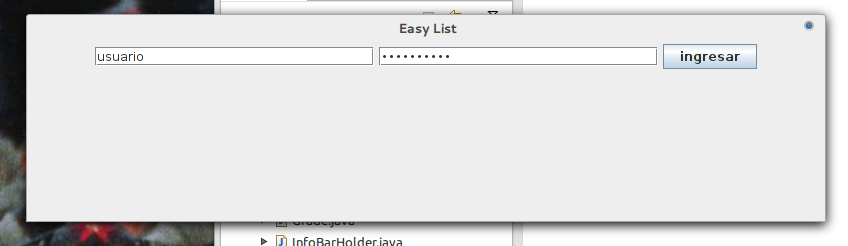
\includegraphics[width=0.85\textwidth]{figuras/ejemplo-a.png}
  \caption{EasyList pantalla inicial.}
  \label{fig:easylist-inicio}
\end{figure}

Esta segunda parte se denomino EasyList, y como se puede ver en la figura \ref{fig:easylist-inicio} permite elegir el nombre de usuario y contraseña con el cual se desea acceder a la base de datos. La base de datos que se usara, en concreto su ubicación debe modificarse en el código al igual que el \dd que se usara.
%

\begin{figure}[h]
  \centering
    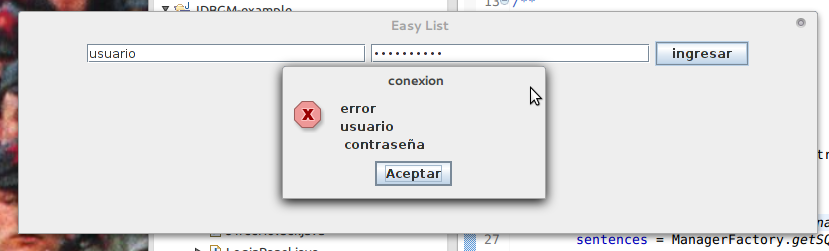
\includegraphics[width=0.85\textwidth]{figuras/ejemplo-b.png}
  \caption{Manejo de errores en EasyList}
  \label{fig:easylist-error}
\end{figure}
%

Como se puede ver en la figura \ref{fig:easylist-error} se incluyo un ejemplo de manejo de excepciones para la vista inicial de \textit{login}. Si se intenta acceder con un nombre de usuario y/o contraseña incorrecto \verb=ManagerFactory= lanzara una excepción pues no va a poder realizar la conexión con motor, por lo que es posible para EasyList capturar esta excepción e informarle a el usuario de la aplicación de dicho error\footnote{En este caso en el mensaje de error se muestra la contraseña en texto plano, algo que siempre debe evitarse por cuestiones de seguridad.} sin que el programa se cuelgue, o sea que el programa posee un modo de recuperarse de algunos errores.

\begin{figure}[h]
  \centering
    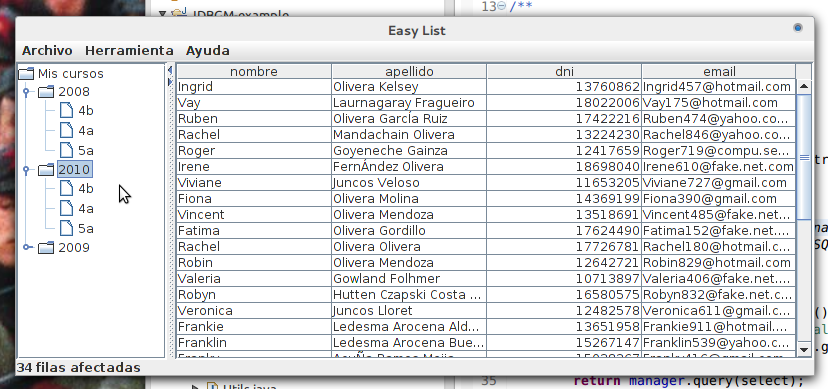
\includegraphics[width=0.85\textwidth]{figuras/ejemplo-c.png}
  \caption{Acceso correcto en EasyList}
  \label{fig:easylist}
\end{figure}

La figura \ref{fig:easylist} muestra como se ve EasyList cuando el usuario pudo ingresar satisfactoriamente sus datos de autenticación. El único elemento realmente funcional de esta interfaz es el árbol de la izquierda que muestra los años que fueron registrados, y por cada año los cursos que fueron registrados por el programa y por cada uno de estos cursos se muestra los alumnos que estaban matriculados en ellos. La lógica de todas estas consultas están contenidas en la clase \verb=DataObtainer= que es la encargada, como su nombre lo dice, de obtener todos los datos de la base de datos. Todas las otras clases que componen esta segunda aplicación son necesarias únicamente para crear la interfaz gráfica.

Al igual que en la aplicación anterior es necesario únicamente cambiar una linea de código para poder usar un \dd distinto. La elección de un motor distinto se podría haber echo dinámicamente  antes de que el usuario ingrese sus credenciales de acceso, pues como ya se menciono anteriormente basta con elegir una constante diferente para indicarle a \verb=ManagerFactory= que se desea usar un motor diferente\footnote{Suponiendo que la ubicación del motor elegido sea siempre la misma que la de los otros motores}, pero como se quería mantener lo mas simple posible la aplicación de ejemplo esto no se implemento.

\section{Resumen}
La importancia de la aplicación de ejemplo es la de mostrar la facilidad con la que se puede migrar de un motor a otro cuando se usa \jj, es por ello que las dos partes que componen el ejemplo son tan simples. Además estas clases que se crearon sirven como guía básica, aparte del manual, para comprender como se usa la librería presentada en este proyecto.

Se puede encontrar todo el código de la aplicación de ejemplo en el repositorio publico \url{https://github.com/nerones/JDBGM-example} alojado en los servidores de \href{https://github.com/}{Github}\footnote{Github es un popular servicio que ofrece alojamiento gratuito para repositorios git que alojen proyectos \textit{open source}}.

%%%%%%%%%%%%%
\backmatter
%%%%%%%%%%%%%
% Adjustments headers
\fancyhead[RO]{\leftmark}
\fancyhead[EL]{}
\addcontentsline{toc}{chapter}{Bibliografía}
\bibliographystyle{plain}
\bibliography{biblio.bib}
%\printindex
\end{document}



%%% Local Variables: 
%%% mode: latex
%%% TeX-master: "tesis"
%%% End: 
